\documentclass[12pt]{article}
\usepackage{nott-titlepage}
\usepackage{graphicx}
\usepackage{float}
\usepackage{amsmath}
\usepackage{hyperref}
% https://tex.stackexchange.com/questions/32598/force-latex-image-to-appear-in-the-section-in-which-its-declared
% https://tex.stackexchange.com/questions/279/how-do-i-ensure-that-figures-appear-in-the-section-theyre-associated-with
\usepackage[section]{placeins}
\usepackage{listings}
\usepackage{tikz}
\usetikzlibrary{shapes,arrows,positioning}

\title{EEEE3112 Coursework 2 Inverter Design}
\author{Tan Hong Kai}
\date{May 13, 2024}
\studentid{20386501}
\module{EEEE3112 Power Electronic Applications and Control}
\department{Department of Electrical and Electronics Engineering}

\begin{document}
\maketitle

\section{Introduction}

This coursework explores the design of DC to AC inverter.
The inverter is a single-phase grid connected inverter facing a solar power network.
The design specification of the inverter is shown in table \ref{tab:design-spec}.

\begin{table}[ht]
    \caption{Design Specification of the Inverter}
    \label{tab:design-spec}
    \centering{}
    \begin{tabular}{l l  l}
        \hline
        Specification/Term                  & Symbol      & Value  \\
        \hline
        DC Voltage                          & $V_{DC}$    & 600 V  \\
        AC RMS Voltage                      & $V_{AC}$    & 240 V  \\
        AC Current Ripple (peak-peak)       & $\Delta{I}$ & 0.5 A  \\
        Rated Power                         & $P$         & 3 kW   \\
        Inverter Switching Frequency        & $f_{sw}$    & 20 kHz \\
        Loss in the Inductor at Rated Power & $P_{LOSS}$  & 1\%P W \\
        Reactive Power                      & $Q_{AC}$    & 0 W    \\
        \hline
    \end{tabular}
\end{table}

In this coursework, all the calculations are done in a Matlab live script.
Furthermore, the live script also contains the code for the control design and analysis.
Using a live script allows for quick calculations of values if any changes were made and the built-in markup makes the code organize.
Once the values for the inverter are calculated, the inverter is then modelled and simulated in PLECS to evaluate the performance.

\section{Inductor Design}

The first part of an inverter design is designing the inductor.
The inductor sits between the inverter and the AC grid.
It acts as a filter to the high frequency switching of the inverter.
Furthermore, the inductor acts as a load with low losses allowing power transfer with the grid.

The main components that effects the inductor design is the AC current ripple $\Delta{I}$.
However, there are other components such as the switching period and DC input voltage which are usually fixed.
Formula \ref{eq:inductor} shows how the inductor size is calculated.
Where $T_{s}$ is the switching period $\frac{1}{f_{sw}}$.

\begin{equation} \label{eq:inductor}
    L = \frac{T_{s} V_{DC}}{8 \Delta{I}} = \frac{0.00005 * 600}{8 * 0.5} = 7.5 mH
\end{equation}

Inductors are not ideal and has some resistance in it.
In this coursework, the resistance of the inductor takes up 1\% of the rated power.
It can be calculated using the power loss equation:

\begin{equation}
    \begin{aligned}
        P_{LOSS} & = I^{2} R                \\
        R        & = \frac{P_{LOSS}}{I^{2}}
    \end{aligned}
\end{equation}

Where:

\begin{equation} \label{eq:current-calculation}
    \begin{aligned}
        I       & = \frac{\sqrt{P^{2} + Q_{AC}^{2}}}{V_{AC}} = \frac{\sqrt{3000^{2} + 0^{2}}}{240} = 12.5 A \\
        \varphi & = -\arctan(\frac{Q_{AC}}{P_{AC}}) = -\arctan(0) = 0^{\circ{}}
    \end{aligned}
\end{equation}

Therefore:

\begin{equation}
    R = \frac{0.01 * 3000}{12.5^{2}} = 0.192 \Omega
\end{equation}

\section{Inverter Voltage}

The power delivered by the inverter to the grid is based on the inverter voltage $V_{INV}$.
Inverter voltage is mainly effected by the current delivered $I$ and inductor impedance $Z$.
The inverter voltage can be calculated using formula \ref{eq:v-inv}.
Note that all the values are calculated in the phasor representation.

\begin{equation} \label{eq:v-inv}
    \begin{aligned}
        \dot{Z}       & = \omega{L}j = 2 * \pi * 50 * 7.5m * j = 2.356j \Omega                   \\
        \dot{V}_{INV} & = \dot{I} \dot{Z} + \dot{V}_{AC} = 12.5 * 2.356j + 240 = 240 + 29.452j V
    \end{aligned}
\end{equation}

The time domain equation can be obtained by converting it from the phasor representation.

\begin{equation}
    \begin{aligned}
        V_{INV}       & = \sqrt{240^2 + 29.452^2} = 241.800 V                                                  \\
        \hat{V}_{INV} & = V_{INV} * \sqrt(2) = 341.957 V                                                       \\
        \gamma        & = \arctan(\frac{29.452}{240}) = 6.996^{\circ{}}                                        \\
        V_{INV}(t)    & = \hat{V}_{INV} \sin(\omega{t} + \gamma{}) = 341.957 \sin(\omega{t} + 6.996^{\circ{}})
    \end{aligned}
\end{equation}

\section{Average Time Model}
\label{sec:avg-time-model}

An average time model of the inverter is design.
In this model, the inverter is modelled as a controllable voltage source.
The inverter is then connected to the grid with the inductor calculated in between.
Measurements of the inverter current and AC grid voltage is taken to calculate the power output.
Figure \ref{fig:avg-time-waveform} shows the output wave forms of the inverter and the average output power.

\begin{figure}[ht]
    % https://tex.stackexchange.com/questions/47245/set-a-maximum-width-and-height-for-an-image/47247
    \centering{}
    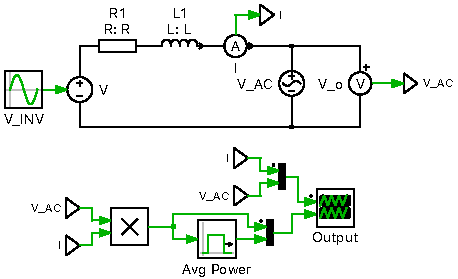
\includegraphics[width=\textwidth, height=0.4\textheight, keepaspectratio]{img/Average Time Model.pdf}
    \caption{PLECS Schematic for Average Time Model}
    \label{fig:avg-time-model}
\end{figure}

The waveforms show that the power output of the inverter matches with the calculated values.
The average power of the inverter is around 2980 W.
This is close to the expected power of $3000 - 1\% * 3000 = 3000 - 30 = 2970$ W.
The difference is due to the precision of the calculated and input values to PLECS.

\begin{figure}[ht]
    % https://tex.stackexchange.com/questions/47245/set-a-maximum-width-and-height-for-an-image/47247
    \centering{}
    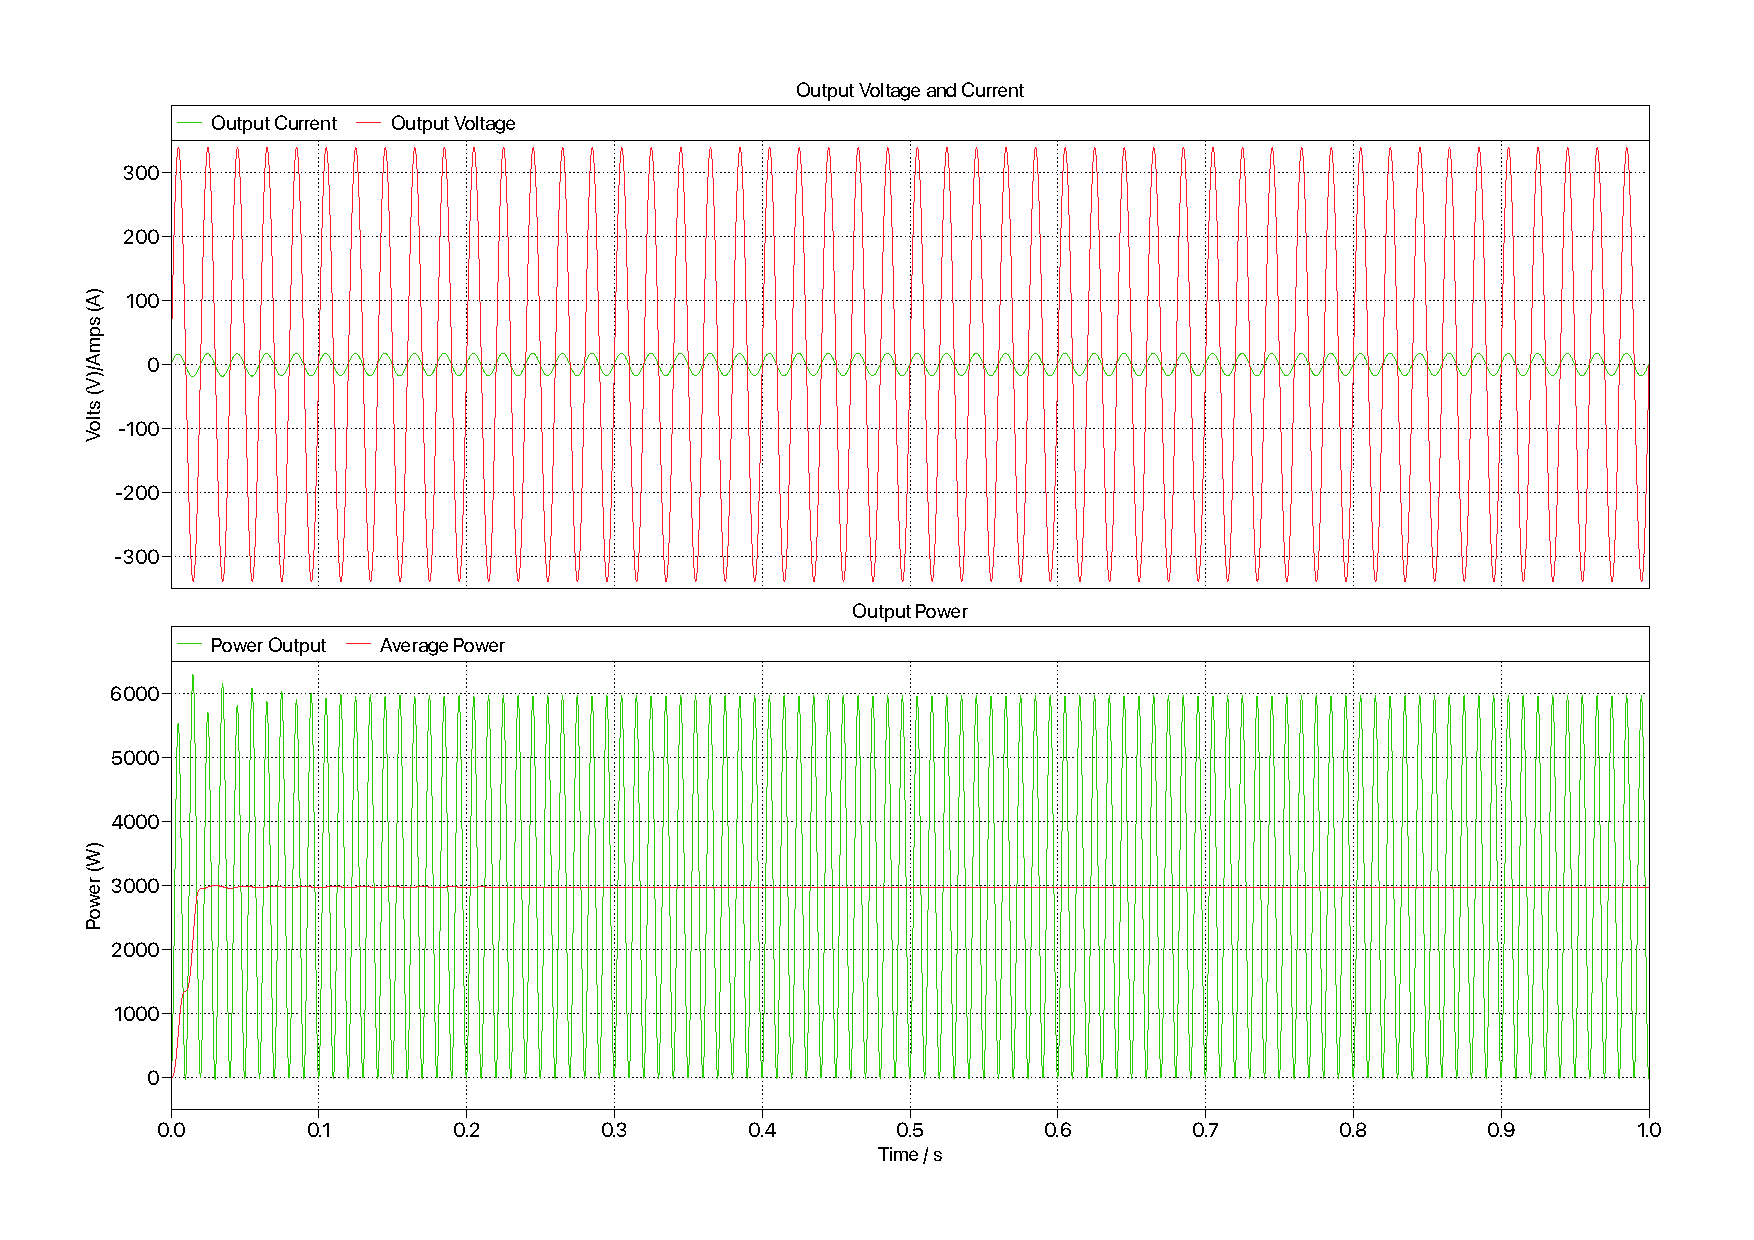
\includegraphics[width=\textwidth, height=0.4\textheight, keepaspectratio]{img/Average Time Power.pdf}
    \caption{Output Waveforms of the Average Time Model Inverter}
    \label{fig:avg-time-waveform}
\end{figure}

\begin{figure}[ht]
    \centering{}
    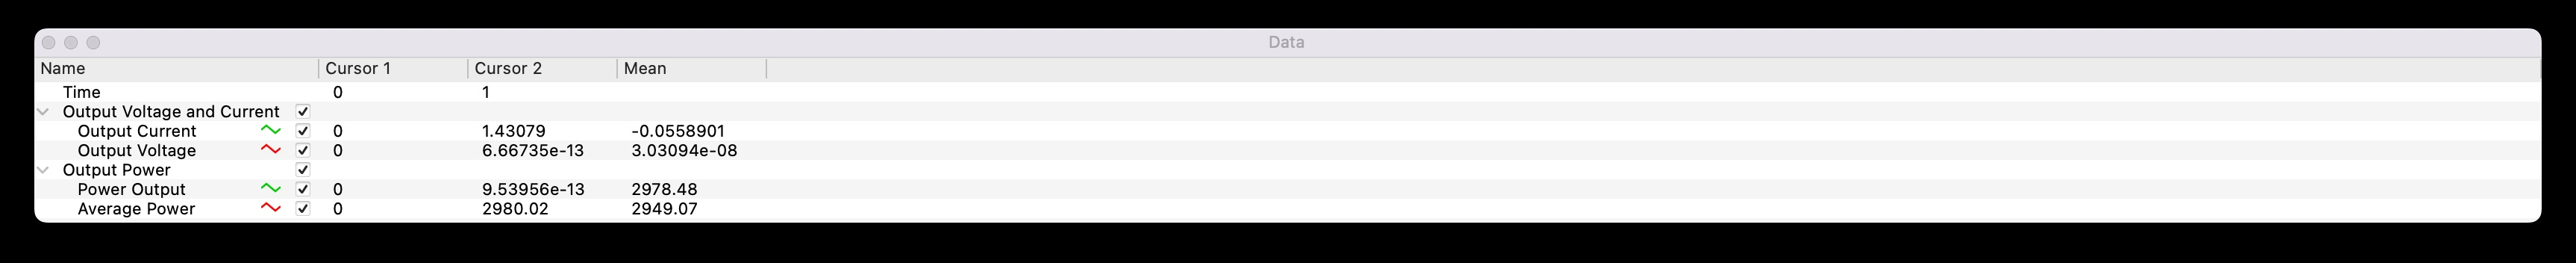
\includegraphics[width=\textwidth, height=0.4\textheight, keepaspectratio]{img/Average Timer Power Cursor.jpg}
    \caption{Measurements from the Average Time Model Waveform}
    \label{fig:avg-time-cursor}
\end{figure}

\section{Switching Model}

A new model is created using a full bridge converter.
This model includes the switching devices (IGBT with diode), DC voltage source and the PWM modulator.
The output of the converter is connected to the grid with the inductor in the middle.

An IGBT is chosen due to the high power application of the inverter.
Furthermore, a freewheeling diode is added to allow for bidirectional current flow.
The IGBT is controlled by the PWM output $G_{B1}$ and $G_{B2}$.

The PWM modulator consists of a comparator for each output.
The negative rail of the comparators are connected to a triangular wave with 20 kHz frequency.
The positive rail of the $G_{B1}$ comparator is connected to $m_1(t)$ while $G_{B2}$ is connected to $m_2(t)$.
Where:

\begin{equation}
    \begin{aligned}
        m_1(t) & = 0.5 + \frac{V_{INV}(t)}{2 V_{DC}} \\
        m_2(t) & = 0.5 - \frac{V_{INV}(t)}{2 V_{DC}} \\
    \end{aligned}
\end{equation}

\begin{figure}[ht]
    \centering{}
    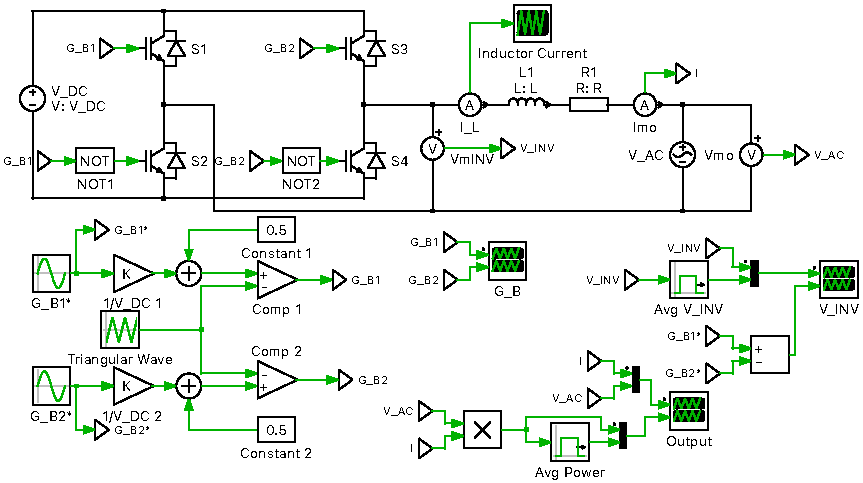
\includegraphics[width=\textwidth, height=0.4\textheight, keepaspectratio]{img/Switching Model.pdf}
    \caption{PLECS Schematic for the Switching Model}
    \label{fig:switching-model}
\end{figure}

In figure \ref{fig:switching-waveform} and \ref{fig:switching-cursor}, the output current and voltage is measured, and the power is calculated.
The calculated average power output is the same as the one in the \hyperref[sec:avg-time-model]{average time model}.

\begin{figure}[ht]
    \centering{}
    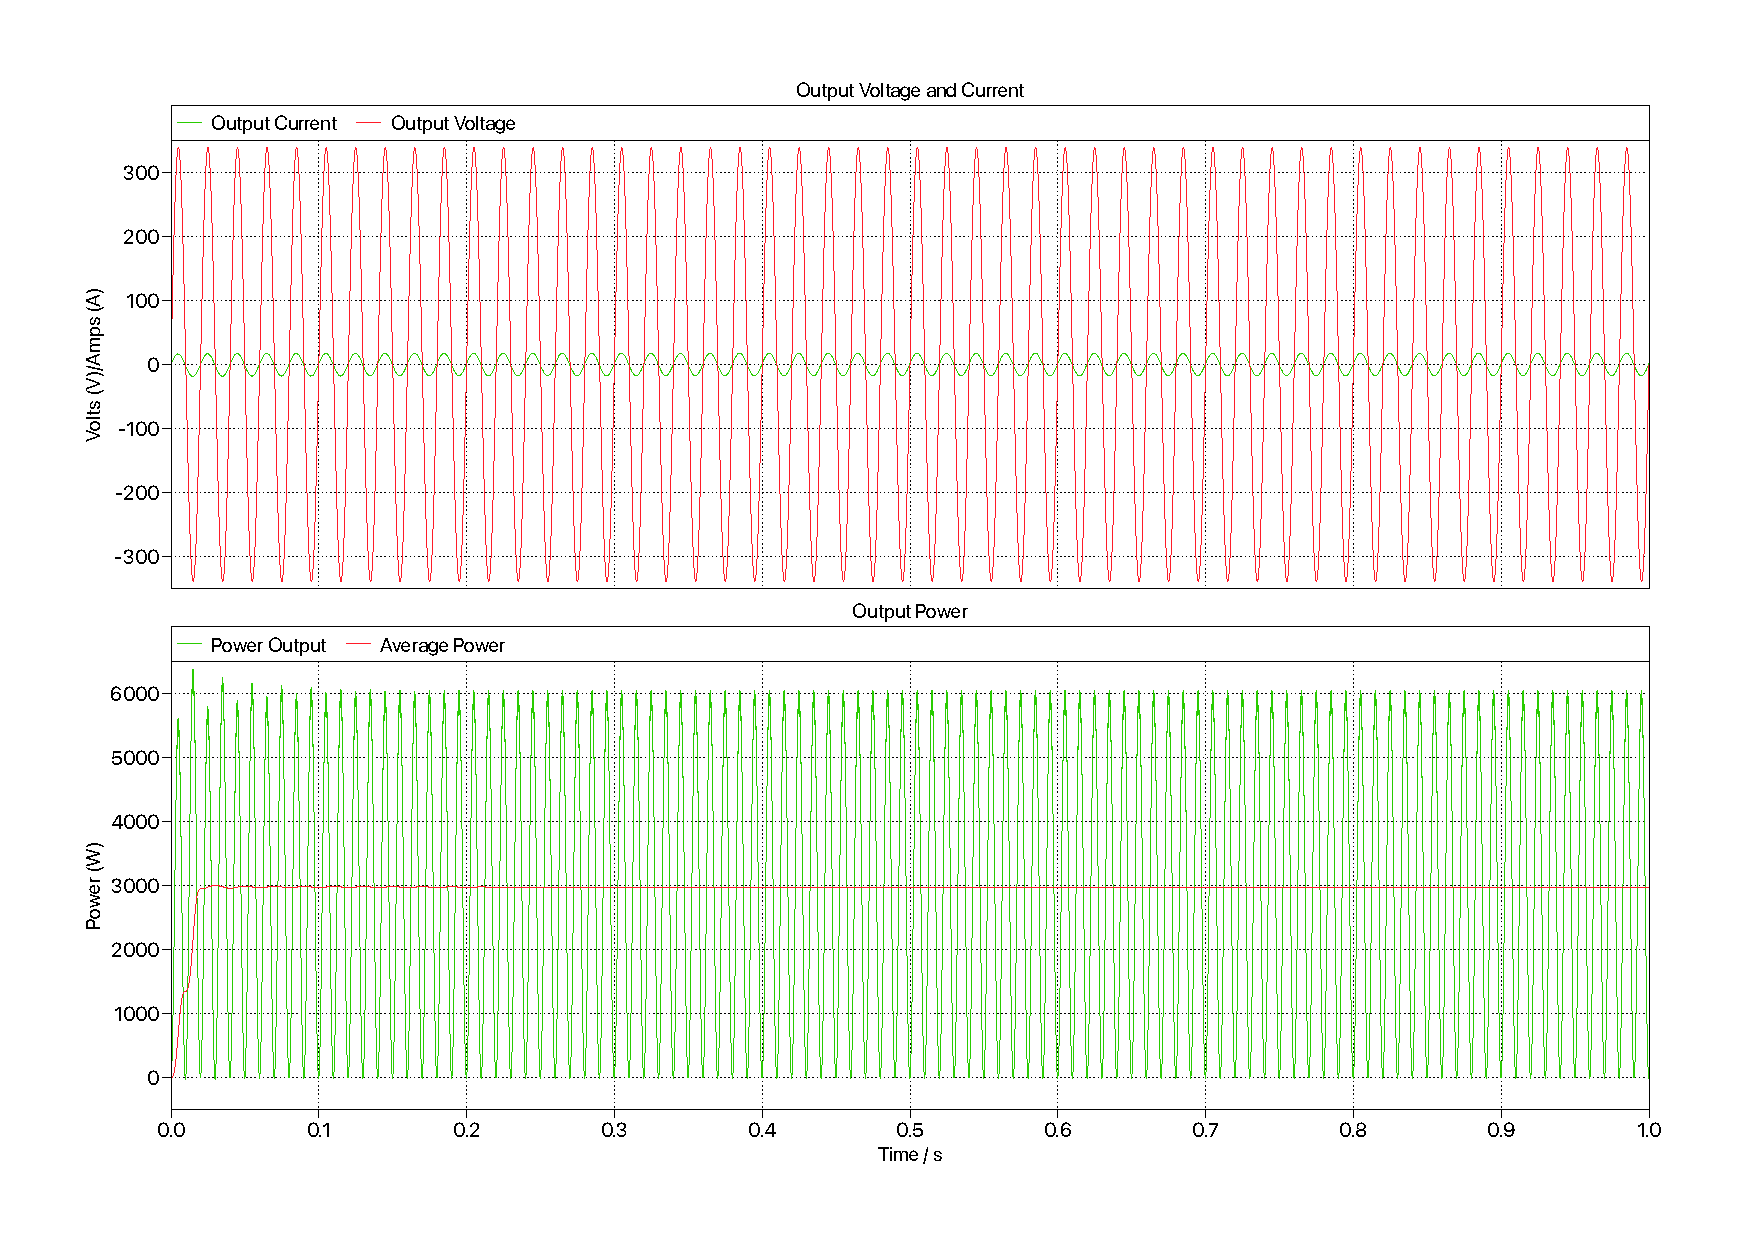
\includegraphics[width=\textwidth, height=0.4\textheight, keepaspectratio]{img/Switching Power.pdf}
    \caption{Output Waveforms of the Switching Model Inverter}
    \label{fig:switching-waveform}
\end{figure}

\begin{figure}[ht]
    \centering{}
    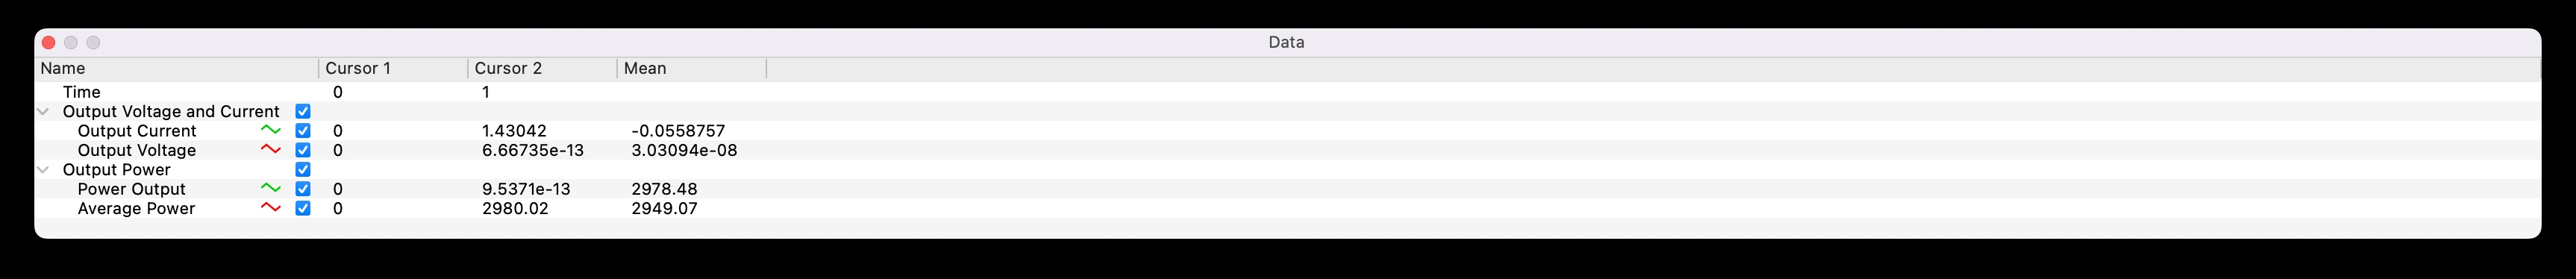
\includegraphics[width=\textwidth, height=0.4\textheight, keepaspectratio]{img/Switching Power Cursor.jpg}
    \caption{Measurements from the Switching Model Waveform}
    \label{fig:switching-cursor}
\end{figure}

Other than output power, the inverter voltage is measured and compared to the voltage demand.
The inverter voltage PWM wave-form is averaged over the switching frequency to show the low frequency component.
In figure \ref{fig:switching-inverter-voltage}, the wave-forms shows that the inverter voltage is able to keep up with the voltage demand generated by the PWM modulator.

To further analyse the inverter voltage, a Fourier analysis is performed.
The Fourier spectrum \ref{fig:switching-fourier} shows that the PWM output have two main frequency spikes.
The first spike occurs at around 0 Hz.
This is due to the low frequency component of the output at 50 Hz.
The value is not at 50 Hz due to the resolution of the frequency axis when sampling for FFT.
The second frequency spike occurs at about 40 kHz.
This is 2 times of the switching frequency.
The inverter output voltage consists of the combination of two half bridges switching at 20 kHz.
When the output of both half bridge is combined, the 20 kHz harmonics add up to 40 kHz causing the frequency spike at the Fourier analysis.

\begin{figure}[ht]
    \centering{}
    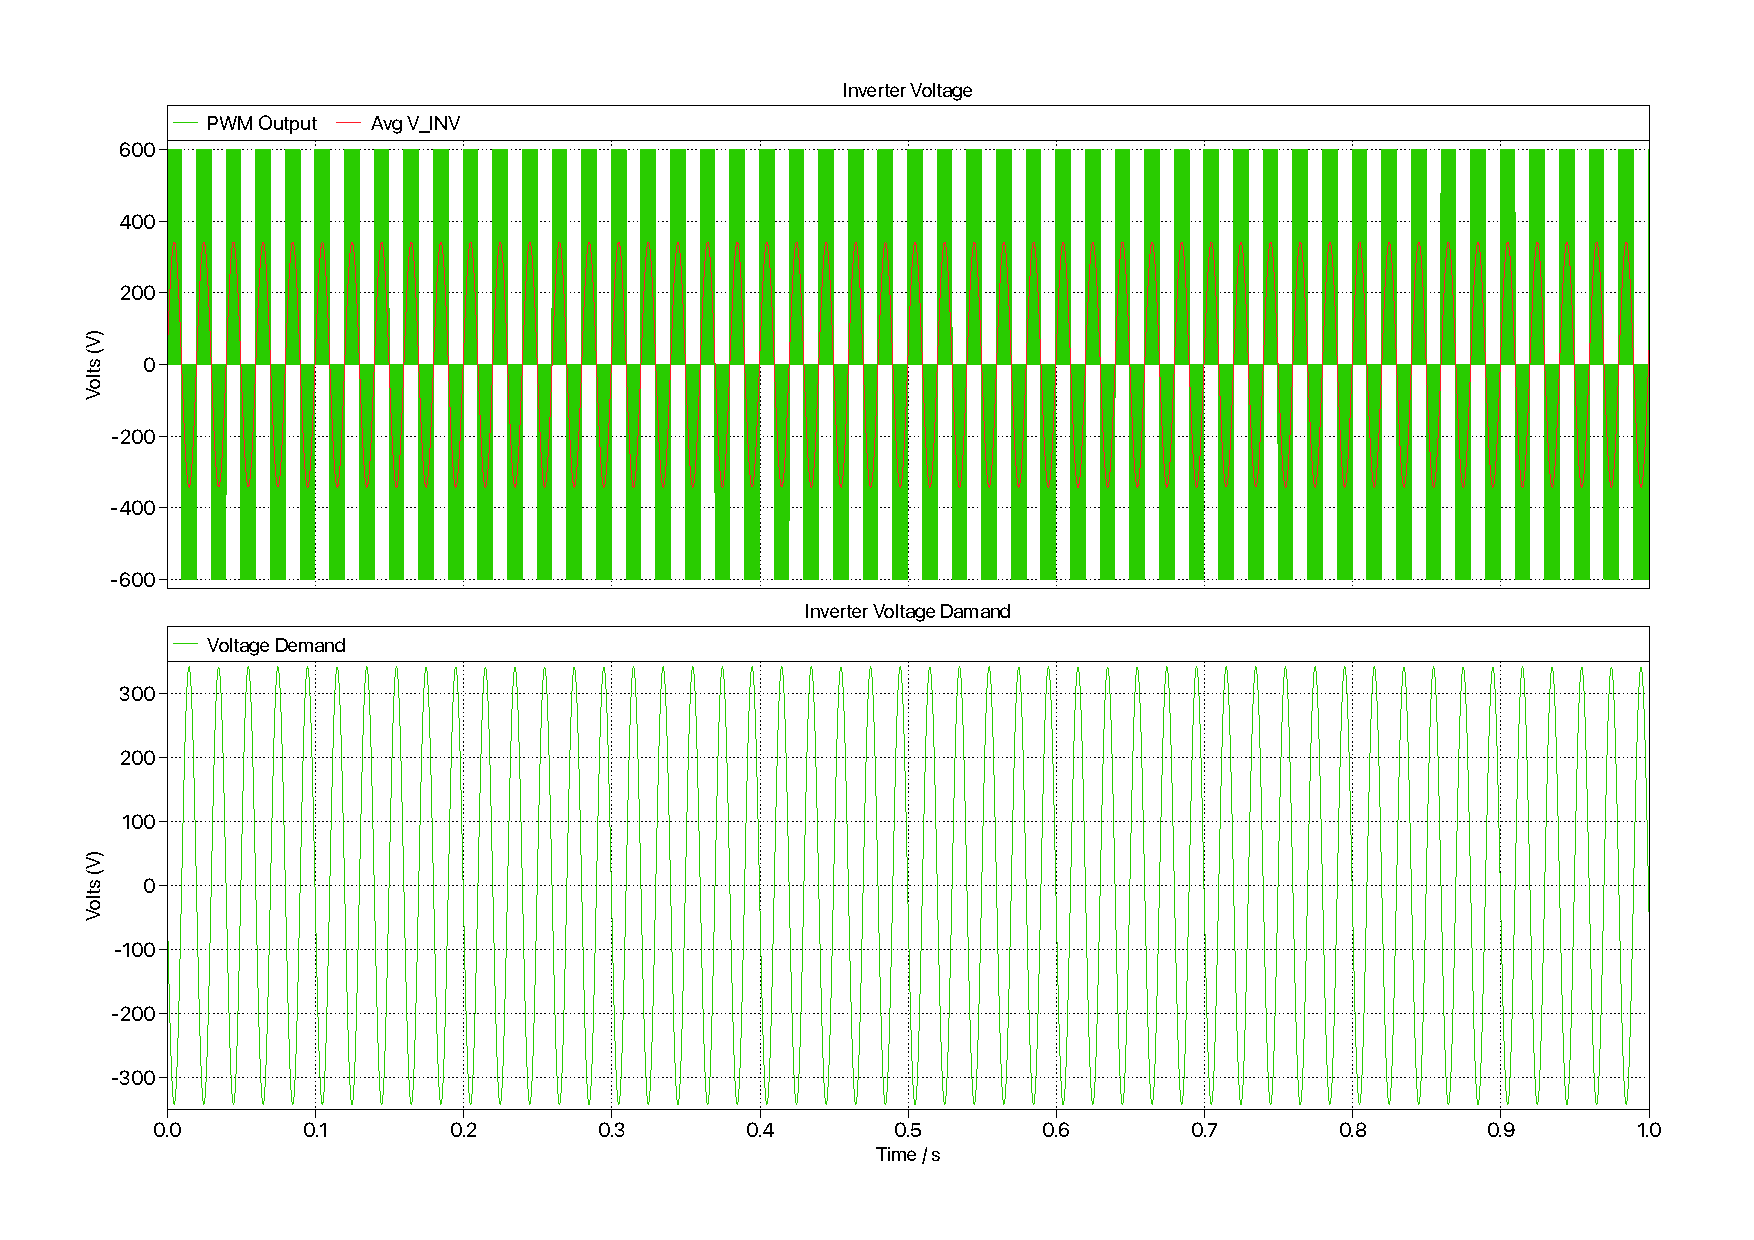
\includegraphics[width=\textwidth, height=0.4\textheight, keepaspectratio]{img/Switching Inverter Voltage.pdf}
    \caption{Output Waveforms of the Inverter Voltage}
    \label{fig:switching-inverter-voltage}
\end{figure}

\begin{figure}[ht]
    \centering{}
    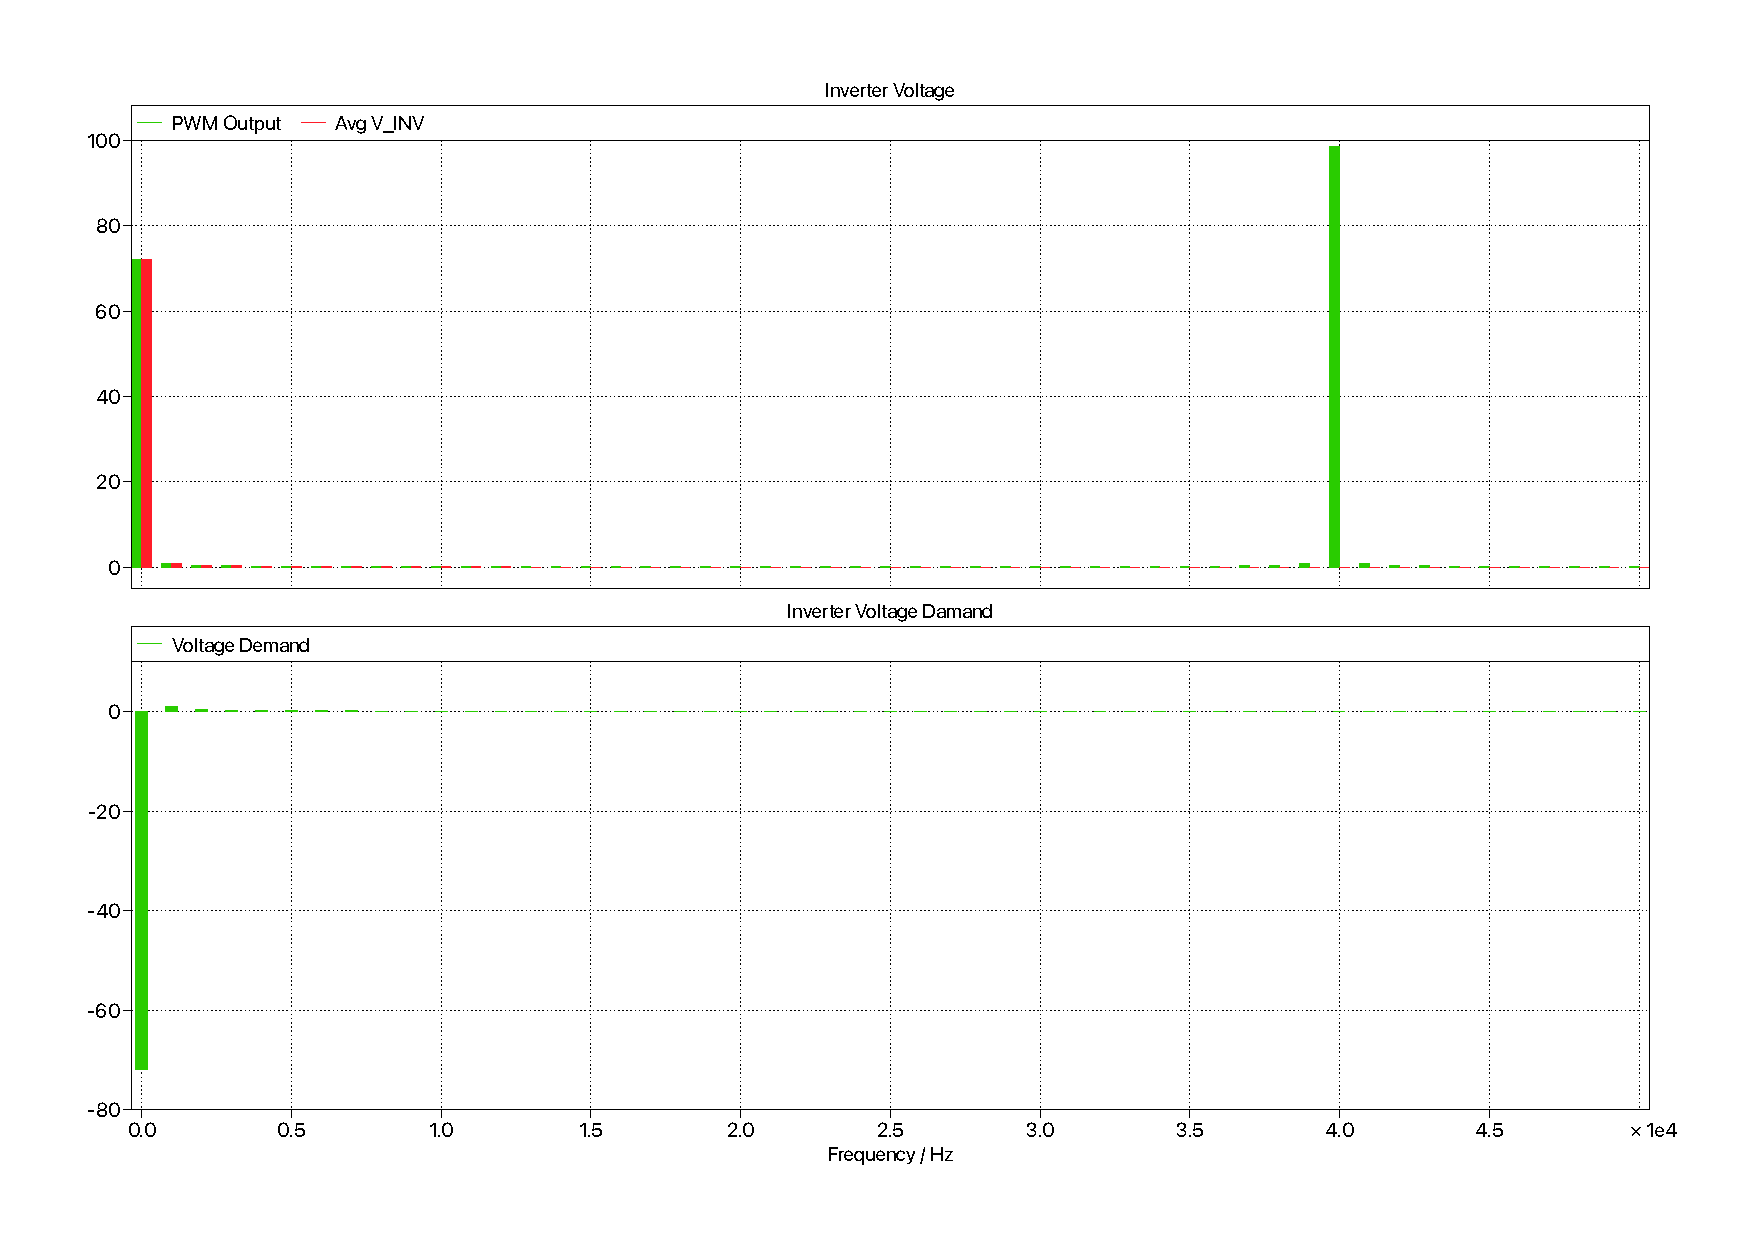
\includegraphics[width=\textwidth, height=0.4\textheight, keepaspectratio]{img/Switching Demand FFT.pdf}
    \caption{Fourier Analysis of the Inverter Voltage}
    \label{fig:switching-fourier}
\end{figure}

The inductor ripple is also considered in the simulation.
Figure \ref{fig:switching-current-ripple} shows the inductor current ripple graph.
From the simulation, the peak to peak current ripple is measured to be 0.491 A which is within the 0.5 A requirement.

\begin{figure}[ht]
    \centering{}
    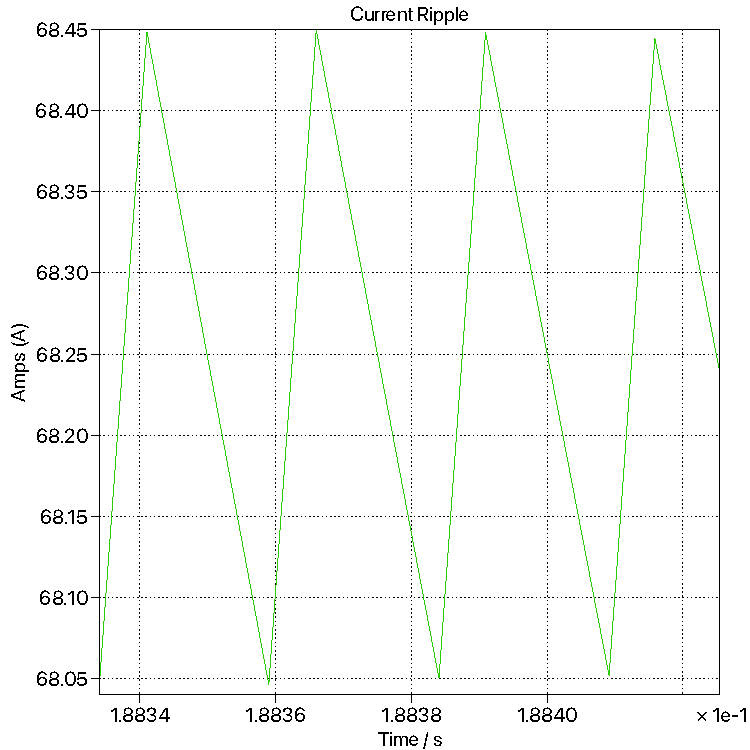
\includegraphics[width=\textwidth, height=0.4\textheight, keepaspectratio]{img/Switching Current Ripple.pdf}
    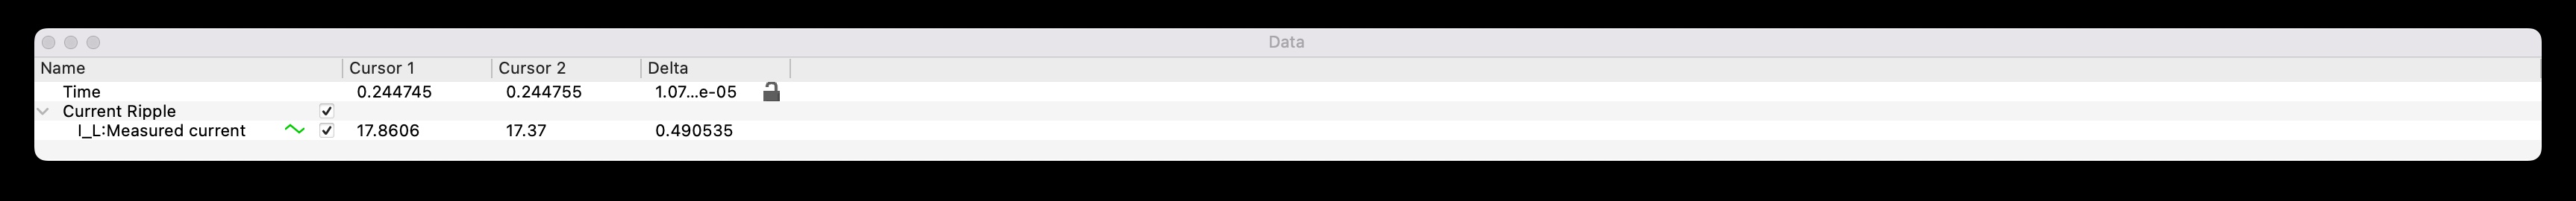
\includegraphics[width=\textwidth, height=0.4\textheight, keepaspectratio]{img/Switching Current Ripple Cursor.jpg}
    \caption{Inductor Current Ripple}
    \label{fig:switching-current-ripple}
\end{figure}

\section{Transfer Function Model}
\label{sec:tf-model}

A transfer function model is also considered.
The entire inverter system is modelled as a plant with the voltage demand as the input and the current to the grid as output.
The transfer function is found to be a first order transfer function effected by the inductor and resistance loss of the inductor.
Equation \ref{eq:plant-tf} shows the plant transfer function of the inverter $G(s)$.

\begin{equation} \label{eq:plant-tf}
    G(s) = \frac{1}{Ls + R} = \frac{1}{0.0075 s + 0.192}
\end{equation}

\begin{figure}[ht]
    \centering{}
    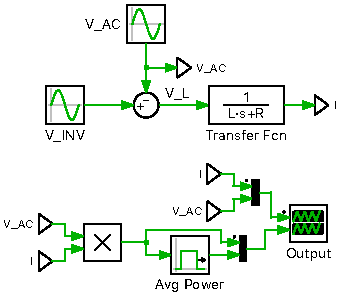
\includegraphics[width=\textwidth, height=0.4\textheight, keepaspectratio]{img/Transfer Function Model.pdf}
    \caption{PLECS Schematic for Transfer Function Model}
    \label{fig:tf-model}
\end{figure}

The power output of the system is measured like the previous two models.
Figure \ref{fig:tf-waveform} shows the output wave form of the model.
As seen in \ref{fig:tf-cursor}, the output power matches the other models.
This shows that the calculated plant transfer function is correct.

\begin{figure}[ht]
    \centering{}
    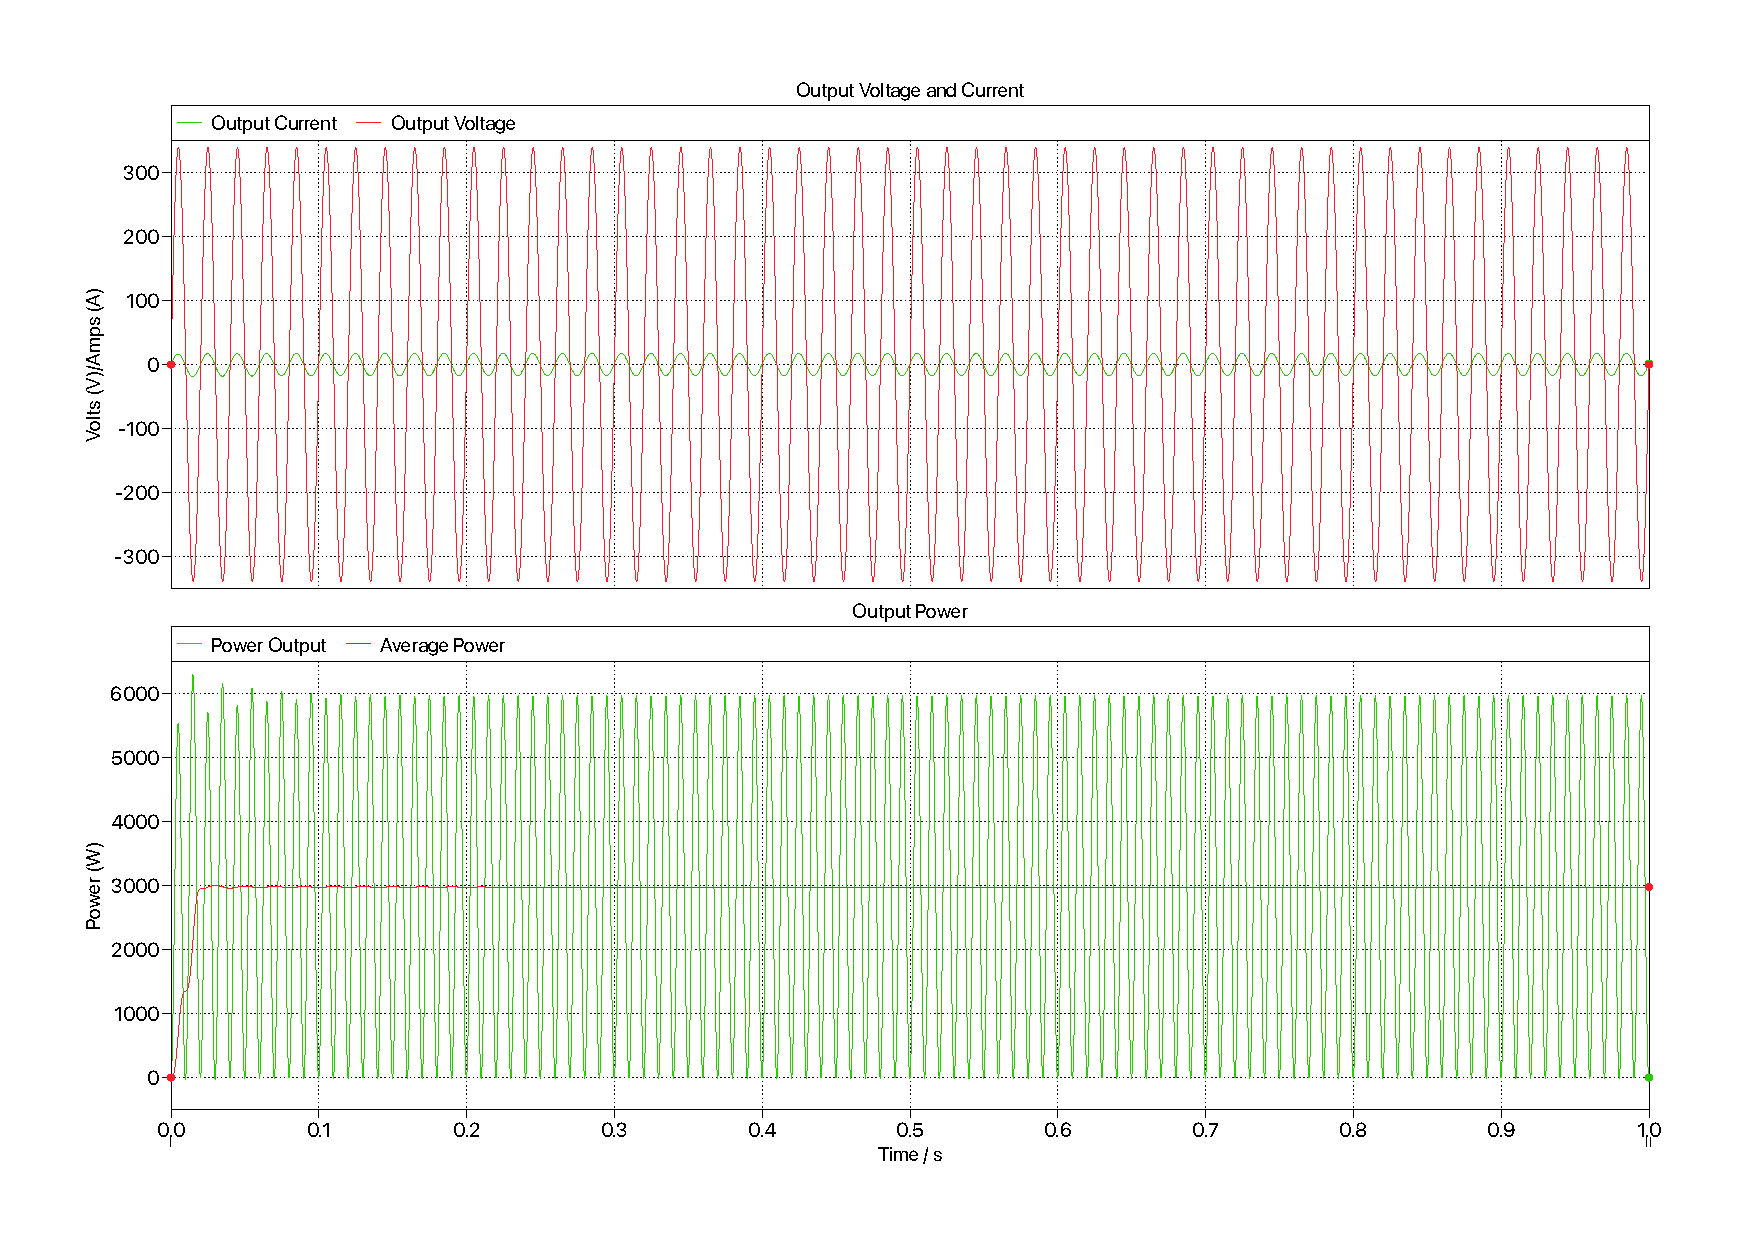
\includegraphics[width=\textwidth, height=0.4\textheight, keepaspectratio]{img/Transfer Function Power.pdf}
    \caption{Output Waveforms of the Transfer Function Model Inverter}
    \label{fig:tf-waveform}
\end{figure}

\begin{figure}[ht]
    \centering{}
    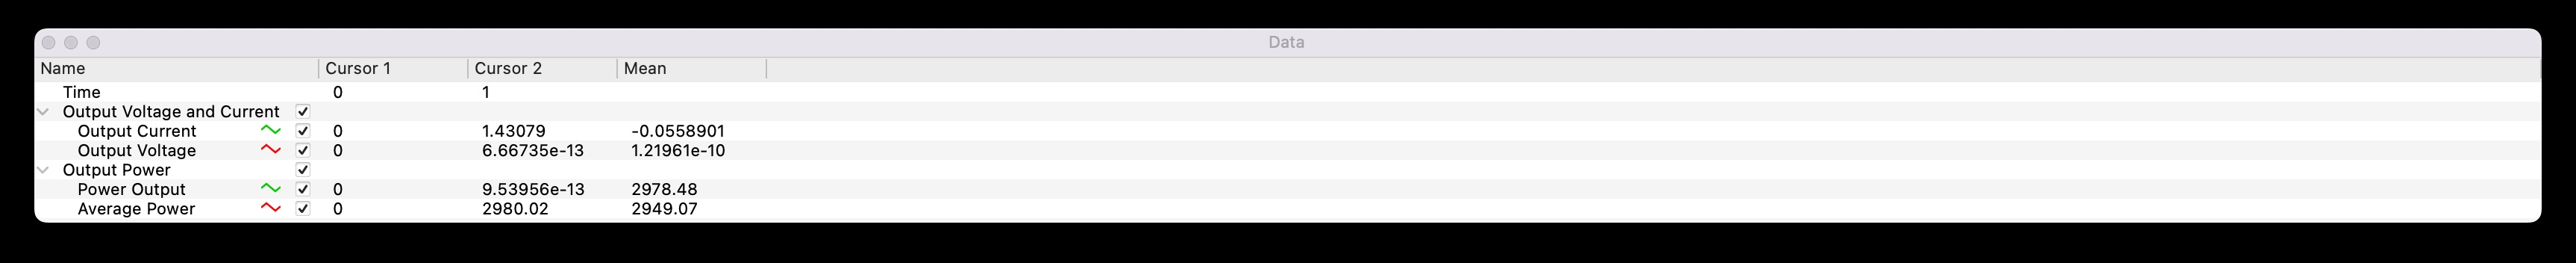
\includegraphics[width=\textwidth, height=0.4\textheight, keepaspectratio]{img/Transfer Function Cursor.jpg}
    \caption{Measurements from the Transfer Function Model Waveform}
    \label{fig:tf-cursor}
\end{figure}

\section{Continuous Current Control Model}
\label{sec:cont-cc-model}

Due to the losses in the inductor and various losses not considered in the simulation, the desired power might not be outputted in a real inverter.
A current controller is needed to control the output current from the inverter to reach desired output power.
Using the transfer function found in \ref{sec:tf-model}, a current control block diagram can be created shown in figure \ref{fig:control-block-diagram}.

% https://tex.stackexchange.com/questions/175969/block-diagrams-using-tikz
\tikzstyle{block} = [draw, fill=white, rectangle,
minimum height=3em, minimum width=6em]
\tikzstyle{sum} = [draw, fill=white, circle, node distance=1cm]
\tikzstyle{input} = [coordinate]
\tikzstyle{output} = [coordinate]
\tikzstyle{pinstyle} = [pin edge={to-, thin, black}]

\begin{figure}
    \centering{}
    \begin{tikzpicture}[auto, node distance=2cm,>=latex']
        \node [input, name=input] {};
        \node [sum, right of=input] (sum) {};
        \node [block, right of=sum] (controller) {$C(s)$};
        \node [sum, right=3em of controller, anchor=west] (disturbance) {};
        \node [block, right=3em of disturbance,
            node distance=3cm] (system) {$G(s)$};
        \node [above=2em of disturbance] (V_AC) {$V_{AC}$};

        \draw [->] (controller) -- node {$V_{INV}$} (disturbance) node[anchor=north east]{$+$} node[anchor=south west] {$-$};
        \draw [->] (disturbance) -- node {$V_{L}$} (system);
        \draw [->] (V_AC) -- (disturbance);
        \node [output, right of=system] (output) {};
        \coordinate [below of=disturbance] (measurements);

        \draw [draw,->] (input) -- node {$I^{ref}$} (sum);
        \draw [->] (sum) -- node {$e$} (controller);
        \draw [->] (system) -- node [name=y] {$I$}(output);
        \draw [->] (y) |- (measurements) -| node[pos=0.99] {$-$}
        node [near end] {$I$} (sum);
    \end{tikzpicture}
    \caption{Control Block Diagram}
    \label{fig:control-block-diagram}
\end{figure}

A current controller with a damping factor ($\zeta$) of 0.7 and natural frequency ($f_0$) of 500 Hz is designed.
This specification is chosen such that the current controller would have a good settling and rise time with acceptable overshoot.
The controller is implemented using sisotool in Matlab with the design requirements in mind.
When designing the controller, an assumption is made that the controller operates at high frequency.
Therefore, the disruption cause by the $V_{AC}$ can be ignored.

A PI controller was originally chosen as the controller.
This is due to the step response from the plant having a steady-state error.
However, when tuning the controller in sisotool, the PI controller is unable to reach the design requirement.
Therefore, a PID controller is used instead.
Equation \ref{eq:pid-continuous} shows the transfer function of the controller.

\begin{equation} \label{eq:pid-continuous}
    C(s) = 424 + 7.88e5 \frac{1}{s} + 0.0558 s
\end{equation}

The PID controller is implemented using the PID block in PLECS.
The controller can then be easily implemented by inserting the correct $K_p$, $K_i$ and $K_d$ value.
The PID controller block also has other functions such as anti-windup and filter, these are ignored and left as default value.
Even though the controller can be implemented using transfer function blocks, it is not used due to the improper nature of the controller transfer function which PLECS does not allow.

The error signal for the PID controller is obtained by subtracting the grid current by the reference current.
The reference current is calculated using the desired power, reactive power and grid voltage.
It consists of a Phase-Lock-Loop (PLL) and current calculation blocks.

The PLL is used to recreate the phase of the grid and calculating the AC RMS voltage.
PLL is implemented by using the Single-Phase PLL block.
Some parameters are changed such as the nominal frequency and nominal input voltage.

The current calculation is split into two separate parts, the amplitude calculation and the phase calculation.
Equation \ref{eq:current-calculation} is used to calculate the current from the desired output power ($P_{AC}$), desired reactive power ($Q_{AC}$) and RMS $V_{AC}$.
$P_{AC}$ and $Q_{AC}$ are supplied as constants while the AC RMS voltage is taken from the PLL output.
The resultant reference current can be calculated using the sin/cos output from the PLL shown in equation \ref{eq:ref-current}.

\begin{equation} \label{eq:ref-current}
    I_{ref} = \hat{I} (\sin(\varphi)\cos(\omega{t}) + \cos(\varphi)\sin(\omega{t}))
\end{equation}

Where:

$\sin(\omega{t})$ and $\cos(\omega{t})$ are the sin/cos output from the PLL.

$\varphi$ is the phase of the desired current.

$\hat{I}$ is the peak-to-peak of the desired current.

\begin{figure}[ht]
    \centering{}
    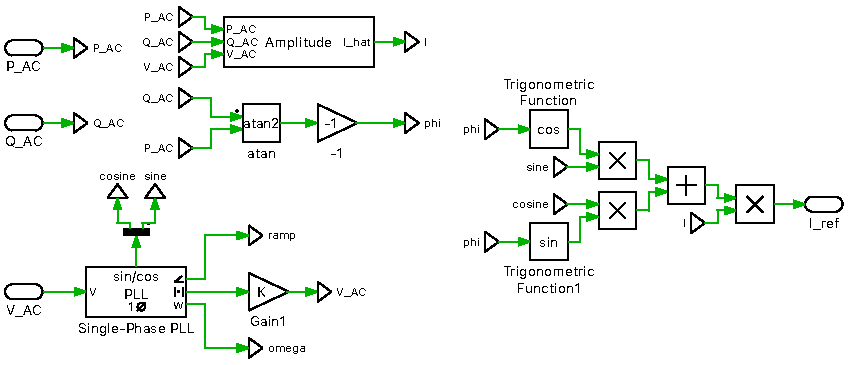
\includegraphics[width=\textwidth, height=0.4\textheight, keepaspectratio]{img/Iref Calculation.pdf}
    \caption{PLECS Schematic for Calculating $I_{ref}$}
    \label{fig:iref-calculation}
\end{figure}

\begin{figure}[ht]
    \centering{}
    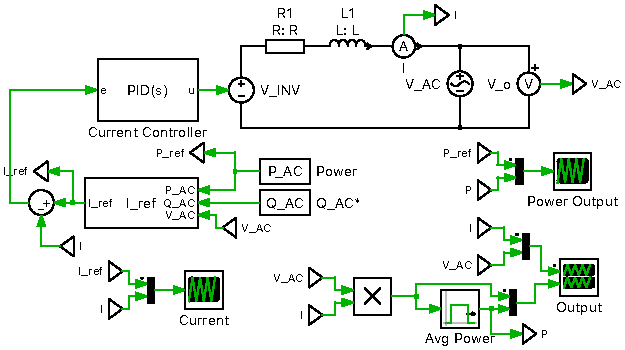
\includegraphics[width=\textwidth, height=0.4\textheight, keepaspectratio]{img/Average Time C Model.pdf}
    \caption{PLECS Schematic for Average Time Continuous Controller Model}
    \label{fig:avg-time-c-model}
\end{figure}

Some modifications to the PWM circuit is made to the switching model.
A zero-order hold with the parameter sample time set to 10 times of the switching time is added.
This is to suppress errors due to the control signal switching too frequently.
A zero-order hold keeps a certain value for the given sample time, reducing the amount of times the signal value changes.

\begin{figure}[ht]
    \centering{}
    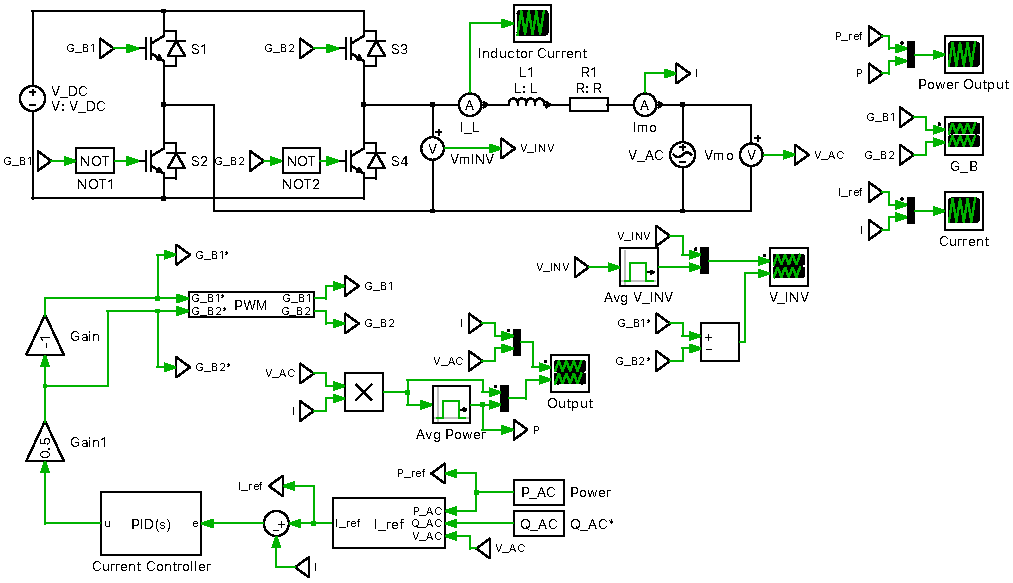
\includegraphics[width=\textwidth, height=0.4\textheight, keepaspectratio]{img/Switching C Model.pdf}
    \caption{PLECS Schematic for Switching Continuous Controller Model}
    \label{fig:switching-c-model}
\end{figure}

To test the performance of the controller two tests are done.
The first test is asking the inverter to generate a power output of 0 W, then step to $\frac{P}{2}$ W, finally resting at $P$ W.
The second test is similar, but the steps are at $-\frac{P}{2}$ W and $-P$ W.
Table \ref{tab:c-transient} shows the steady-state average output power of the inverter.
Figure \ref{fig:avg-time-c-power-positive}, \ref{fig:avg-time-c-power-negative}, \ref{fig:switching-c-power-positive}, and \ref{fig:switching-c-power-negative} shows the transient output power response of the inverter.

\begin{table}[ht]
    \caption{Steady-State Average Power Output of Inverter}
    \label{tab:c-transient}
    \centering{}
    \begin{tabular}{ l l l }
        \hline
        Model        & Desired Power (W) & Output Power (W) \\
        \hline
        Average Time & $0$               & -3.783           \\
        Average Time & $1500$            & 1497.57          \\
        Average Time & $3000$            & 2998.92          \\
        \hline
        Average Time & $0$               & -3.783           \\
        Average Time & $-1500$           & -1505.14         \\
        Average Time & $-3000$           & -3006.49         \\
        \hline
        Switching    & $0$               & -3.840           \\
        Switching    & $1500$            & 1497.52          \\
        Switching    & $3000$            & 2998.88          \\
        \hline
        Switching    & $0$               & -3.840           \\
        Switching    & $-1500$           & -1505.20         \\
        Switching    & $-3000$           & -3006.56         \\
        \hline
    \end{tabular}
\end{table}

\begin{figure}[ht]
    \centering{}
    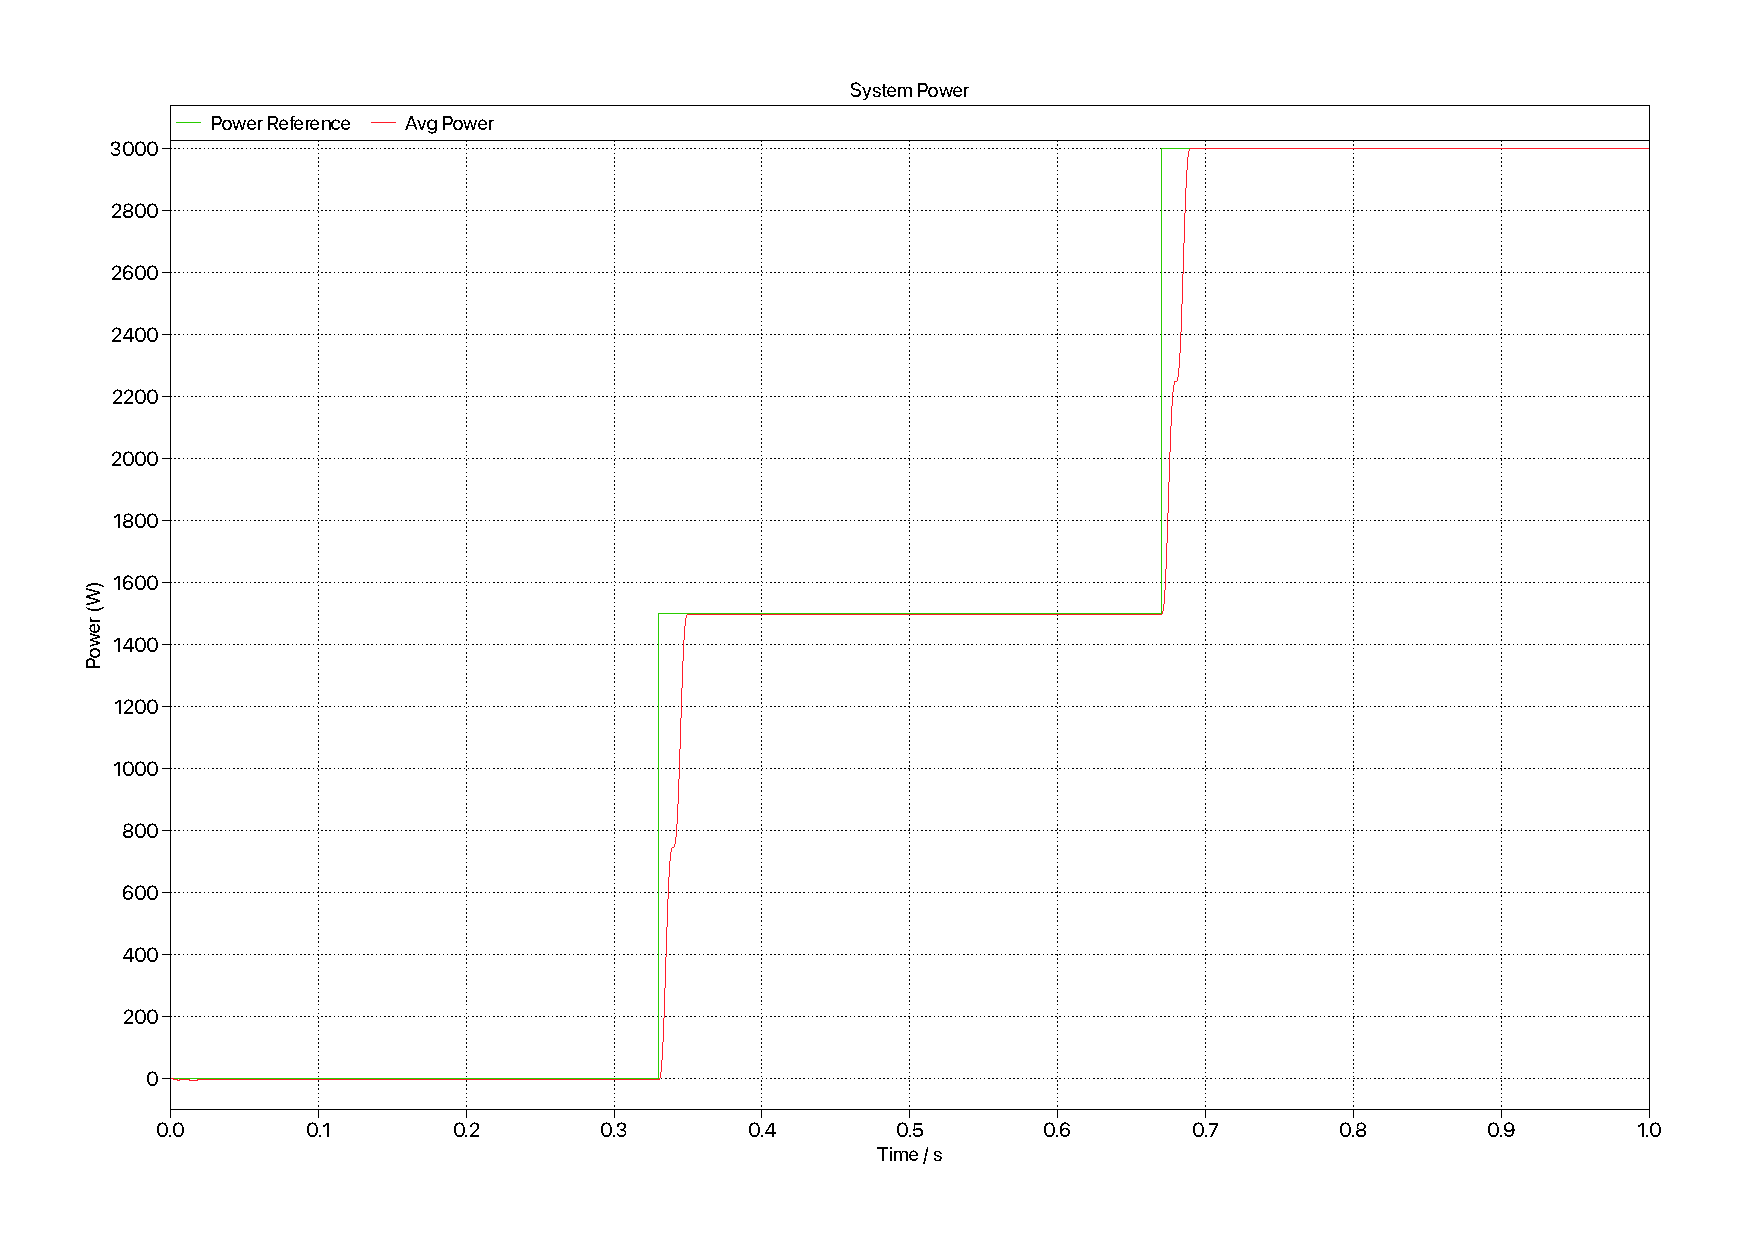
\includegraphics[width=\textwidth, height=0.4\textheight, keepaspectratio]{img/Average Time C Power Positive.pdf}
    \caption{Desired Power vs Output Power Average Time Continuous Controller Positive}
    \label{fig:avg-time-c-power-positive}
\end{figure}

\begin{figure}[ht]
    \centering{}
    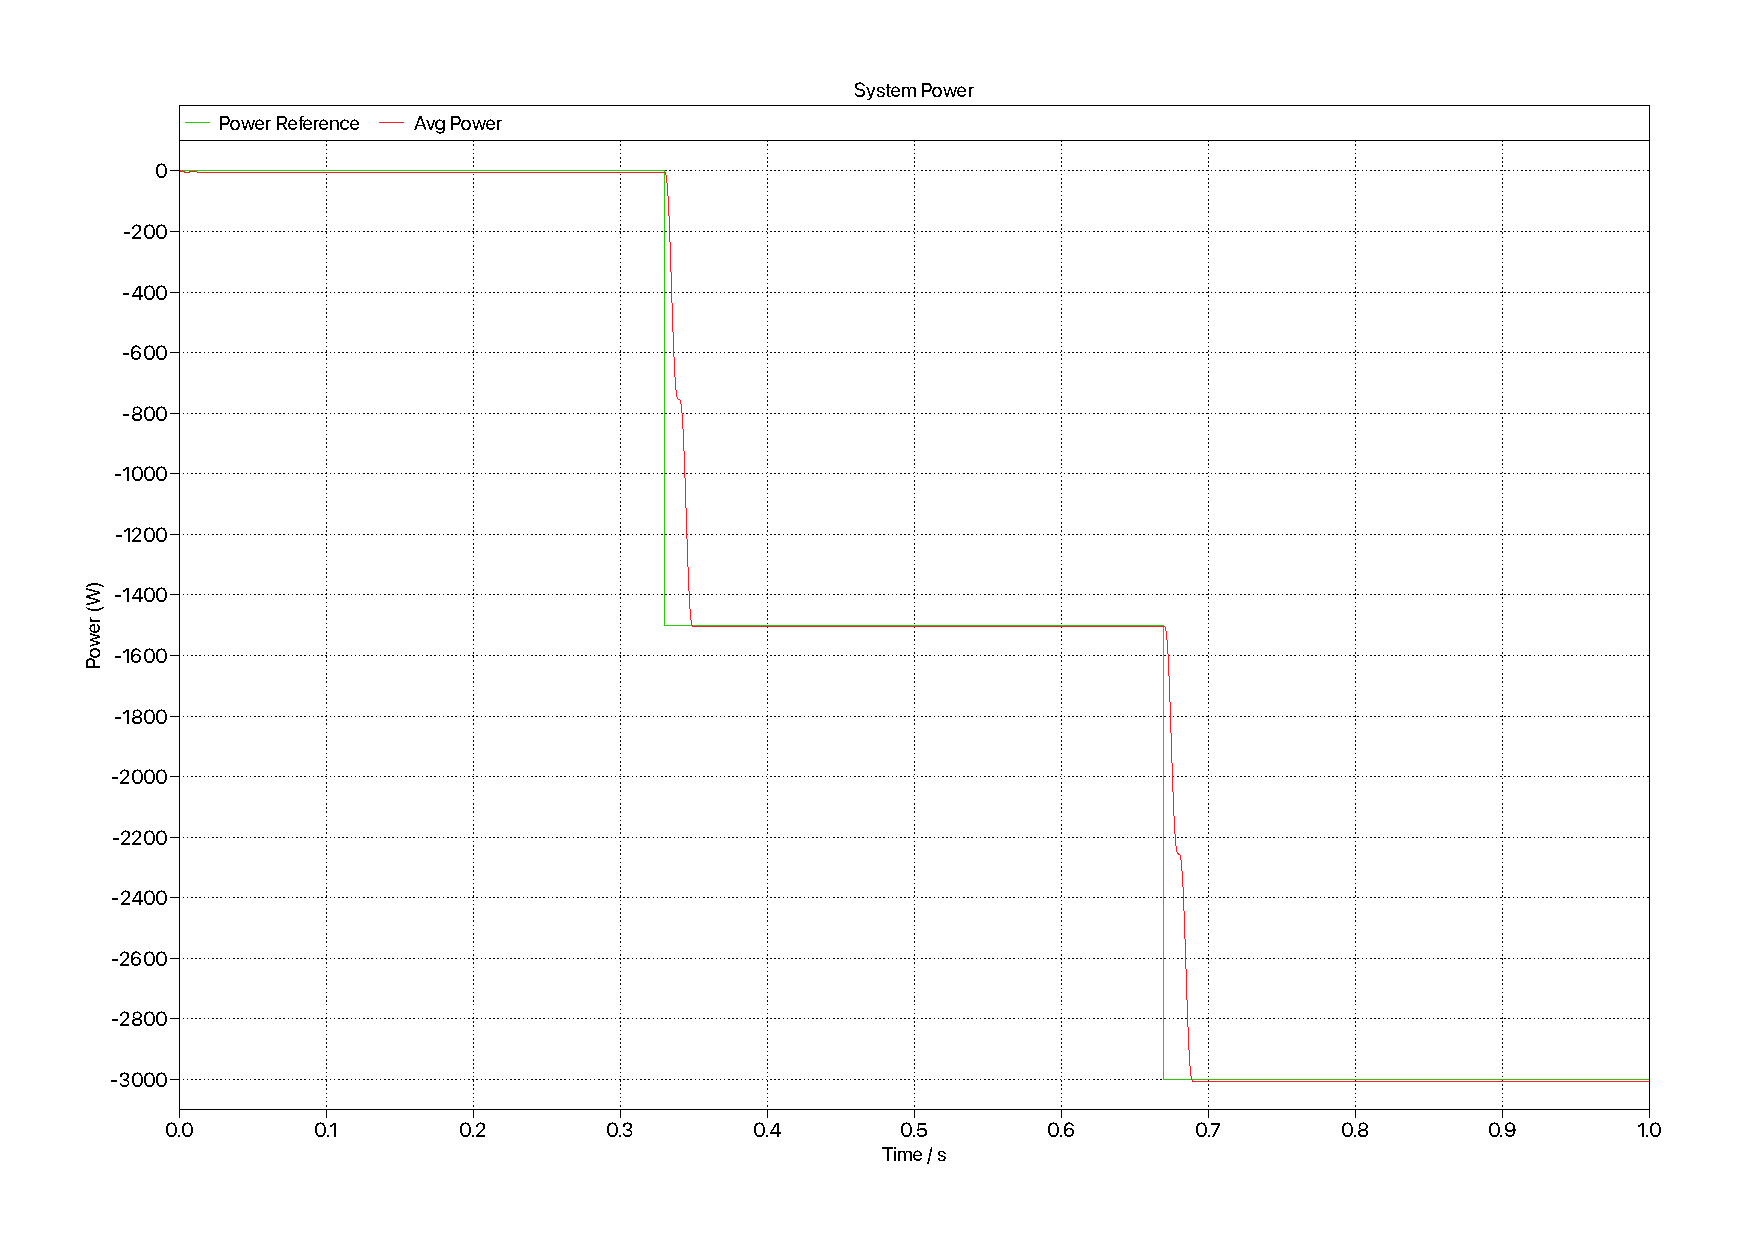
\includegraphics[width=\textwidth, height=0.4\textheight, keepaspectratio]{img/Average Time C Power Negative.pdf}
    \caption{Desired Power vs Output Power Average Time Continuous Controller Negative}
    \label{fig:avg-time-c-power-negative}
\end{figure}

\begin{figure}[ht]
    \centering{}
    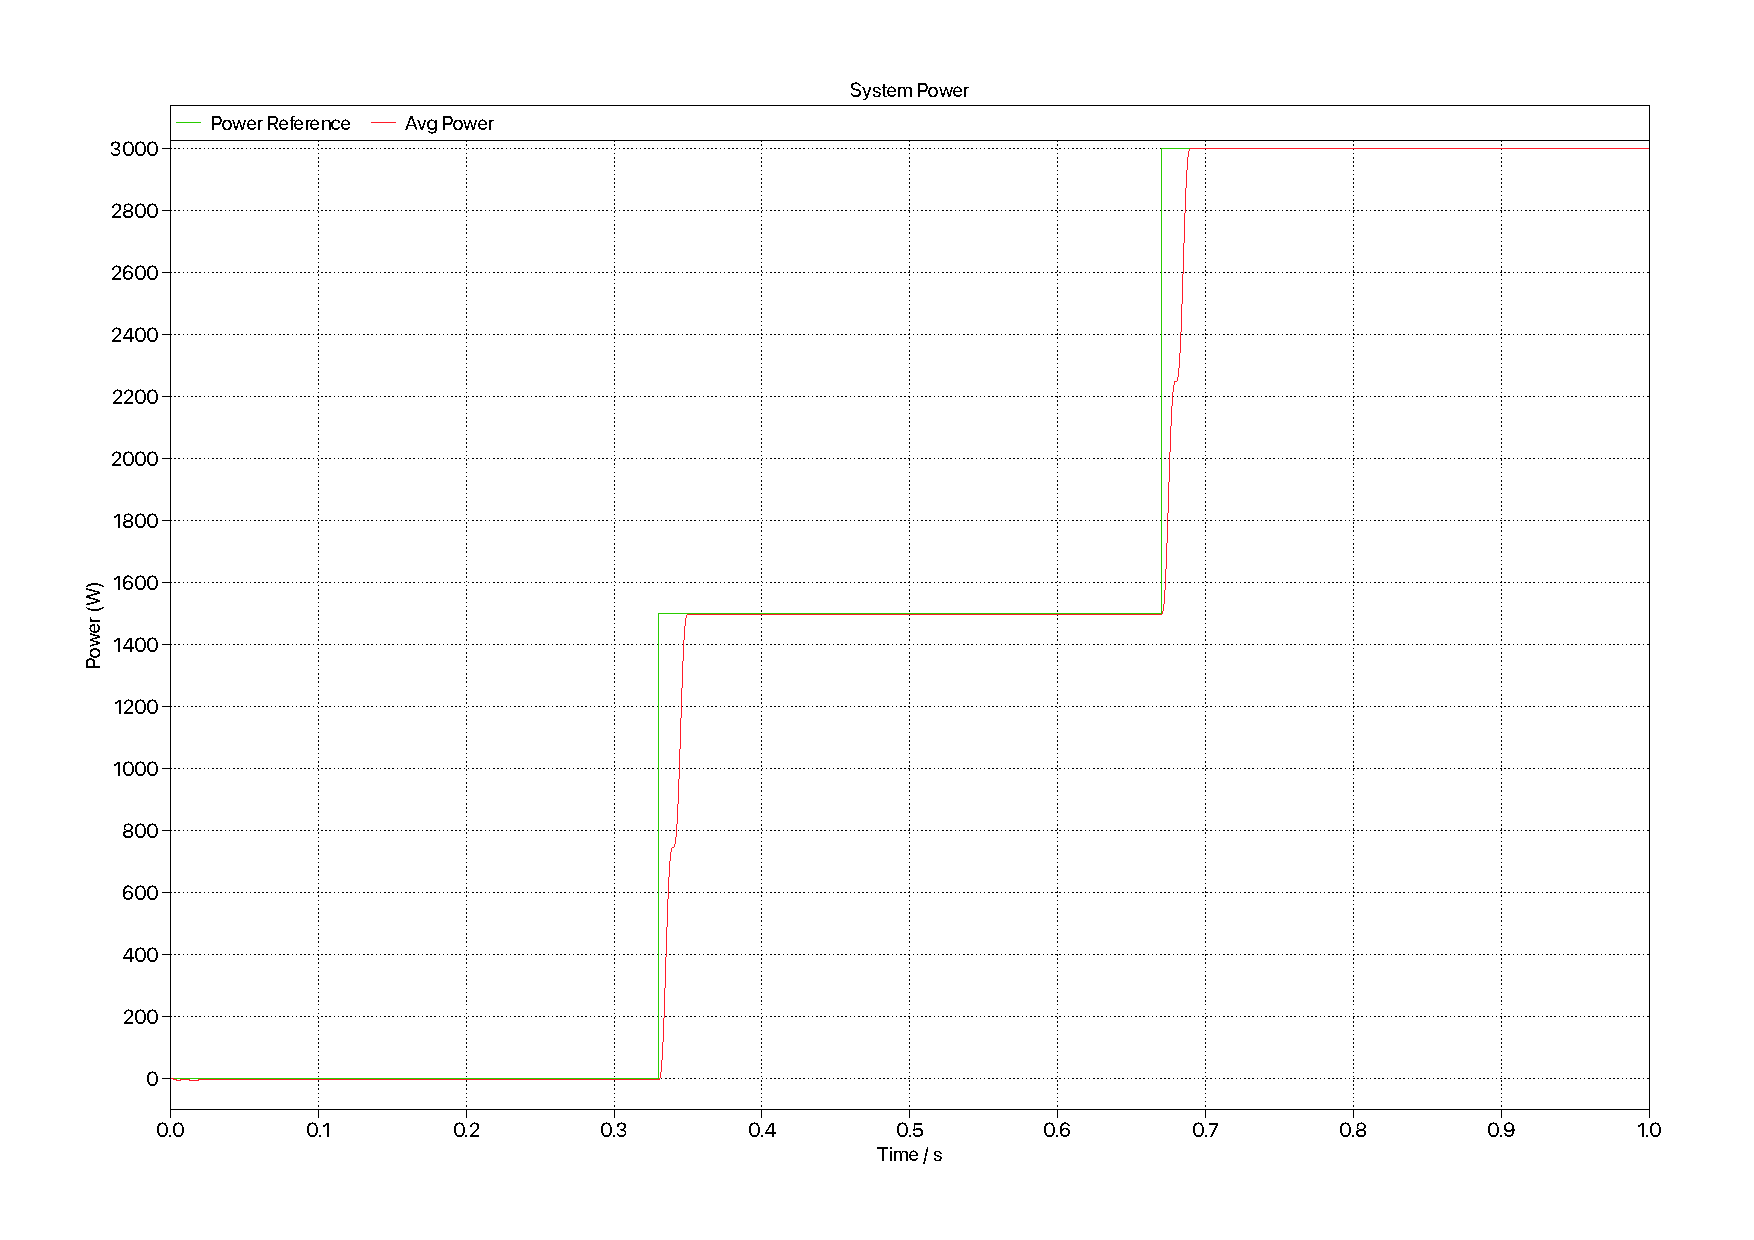
\includegraphics[width=\textwidth, height=0.4\textheight, keepaspectratio]{img/Switching C Power Positive.pdf}
    \caption{Desired Power vs Output Power Switching Continuous Controller Positive}
    \label{fig:switching-c-power-positive}
\end{figure}

\begin{figure}[ht]
    \centering{}
    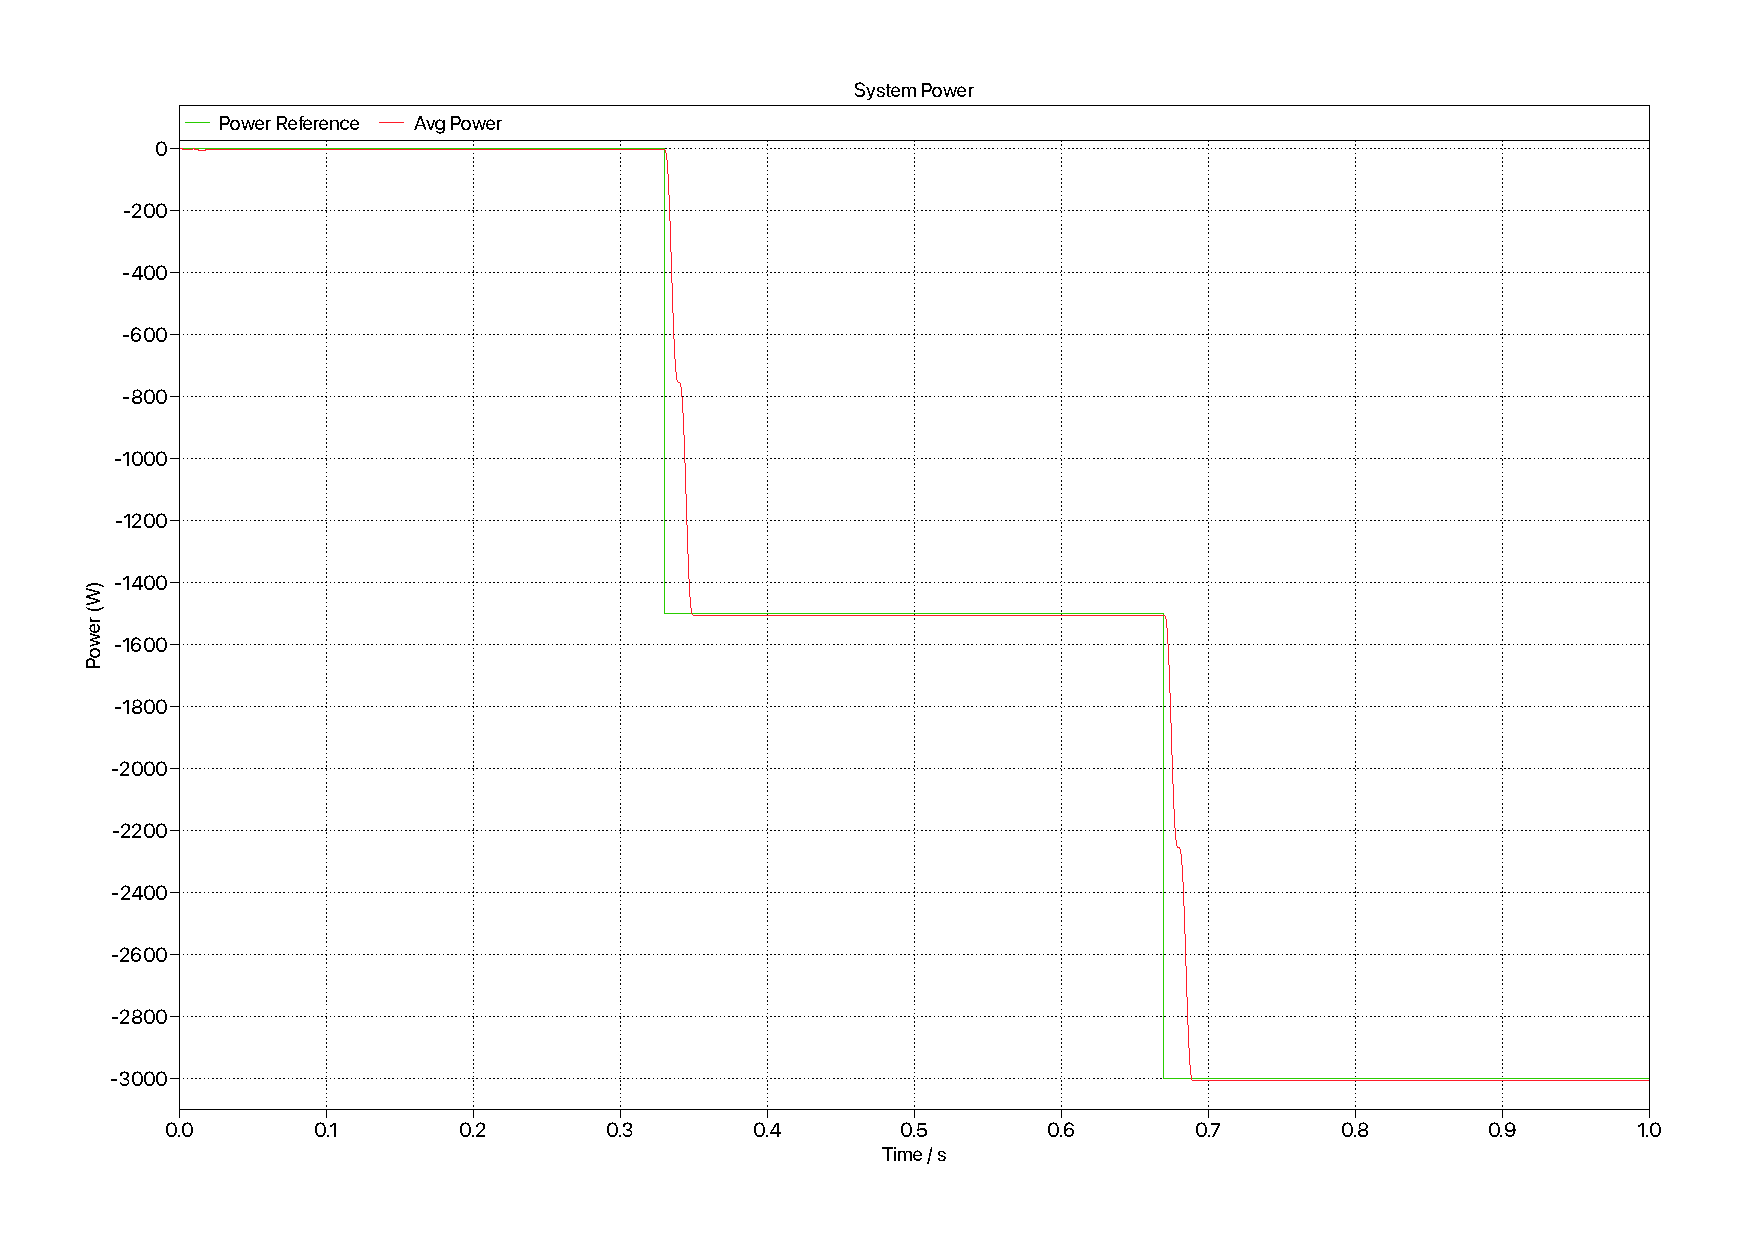
\includegraphics[width=\textwidth, height=0.4\textheight, keepaspectratio]{img/Switching C Power Negative.pdf}
    \caption{Desired Power vs Output Power Switching Continuous Controller Negative}
    \label{fig:switching-c-power-negative}
\end{figure}

As shown in table \ref{tab:c-transient}, the average transient output power is not exactly the same.
This is due to the controller not being able to match the exact current reference.
The output current is similar to the reference current (see \ref{fig:switching-c-current}), but there is some offset.
The offset is mostly cause by the grid voltage.
This is especially true when the power of 0 W.
The grid voltage interfere with the inverter voltage causing a mismatch in current.

Both average time and switching model can follow the reference current.
However, the switching model output current has high frequency ripple caused by the switching.
This is especially obvious when the target power is 0 W, resulting in a sausage like shape.
Figure \ref{fig:switching-c-current-ripple} shows the sausage ripple current in the switching model.

\begin{figure}[ht]
    \centering{}
    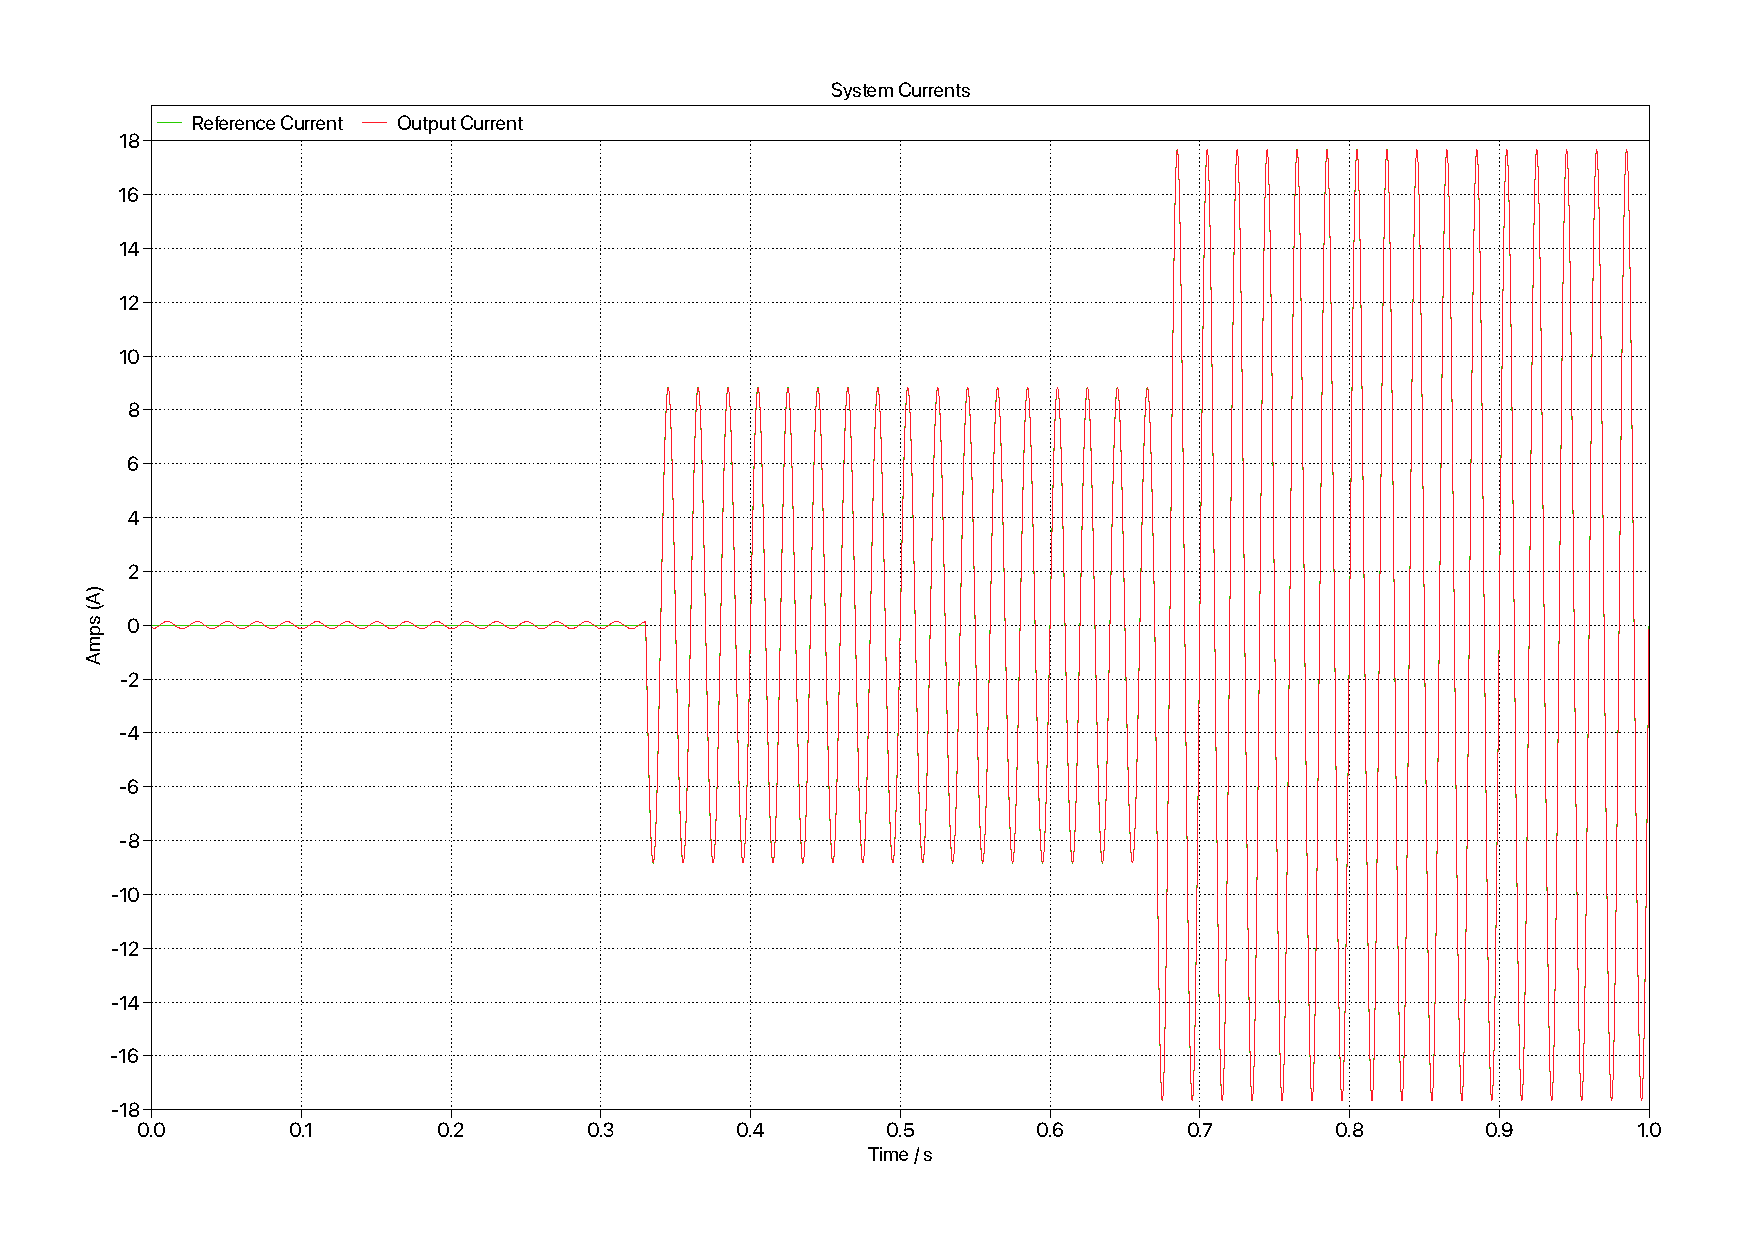
\includegraphics[width=\textwidth, height=0.4\textheight, keepaspectratio]{img/Average Time C Current.pdf}
    \caption{Desired Current vs Output Current of Inverter}
    \label{fig:switching-c-current}
\end{figure}

\begin{figure}[ht]
    \centering{}
    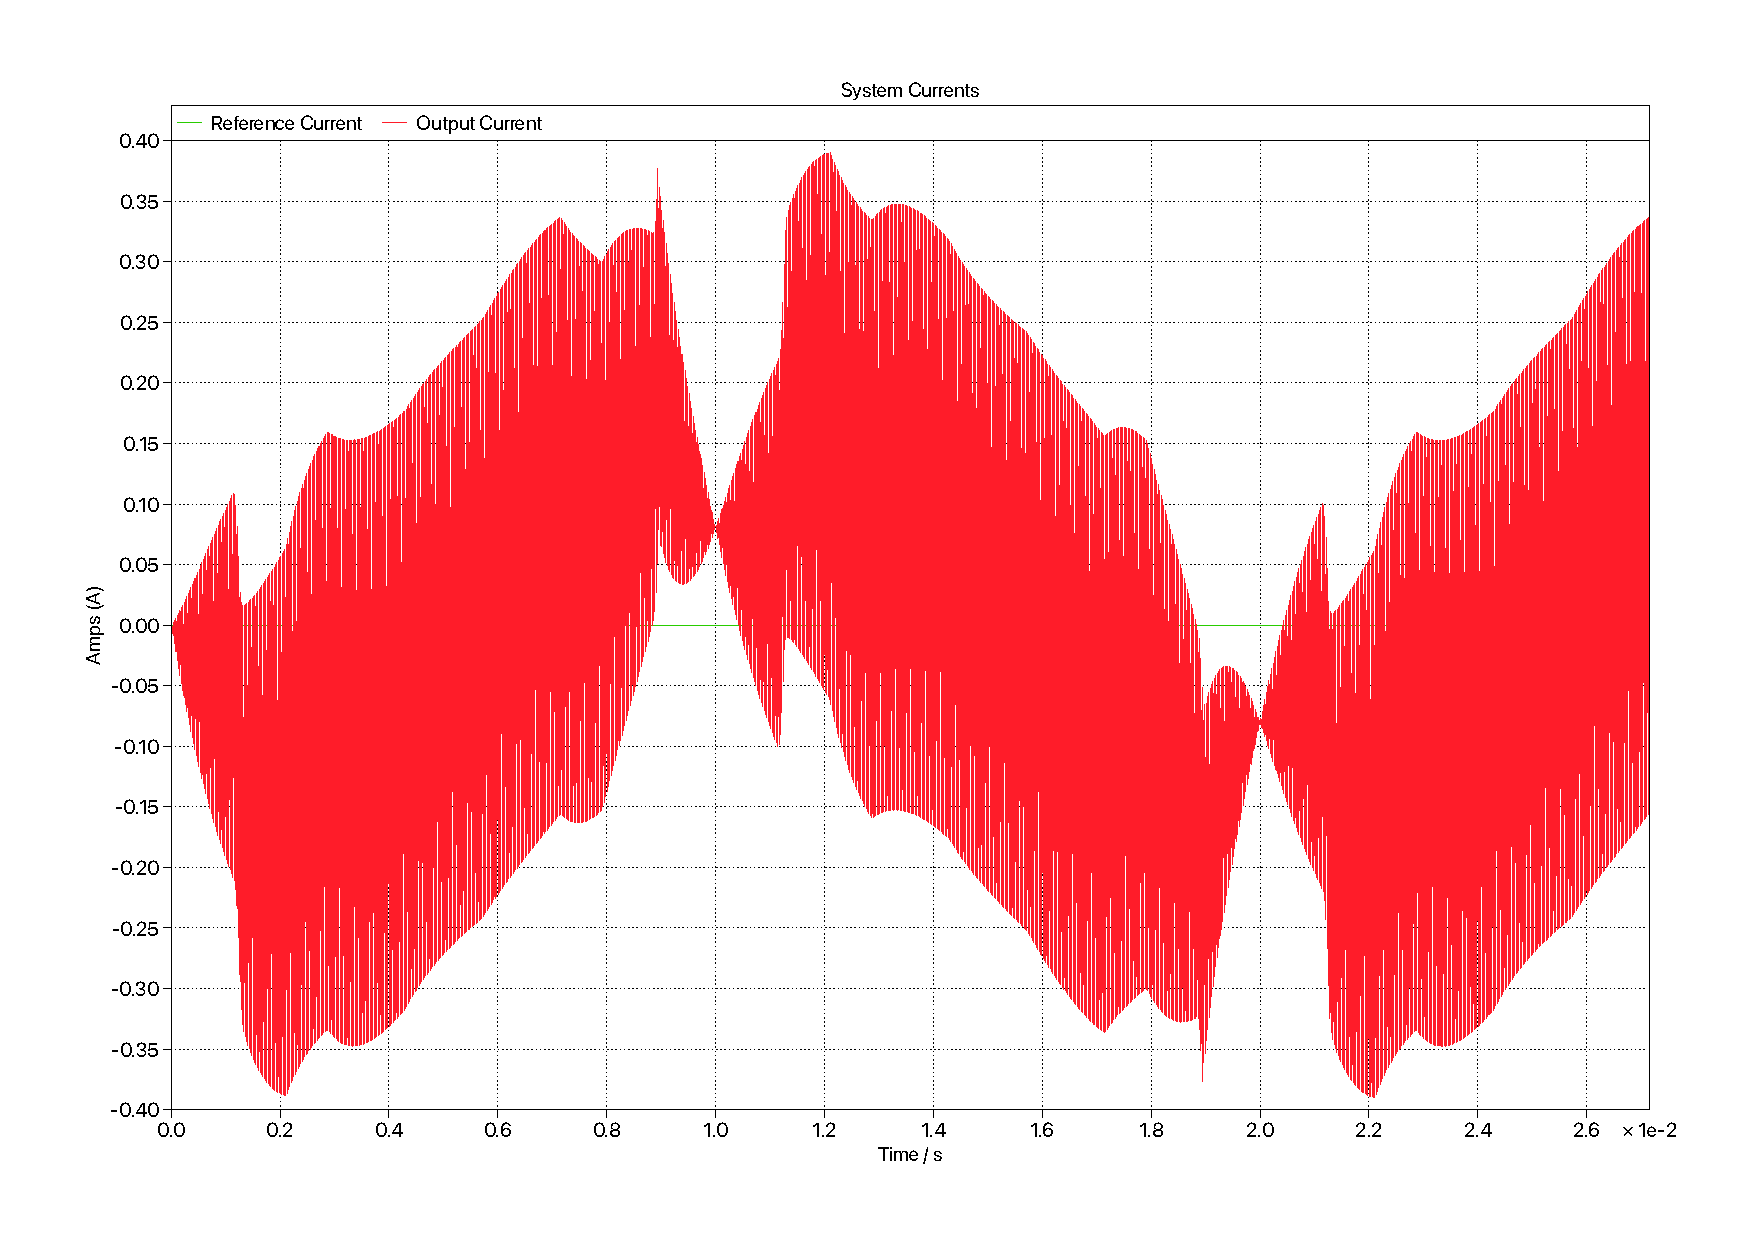
\includegraphics[width=\textwidth, height=0.4\textheight, keepaspectratio]{img/Switching C Current Ripple.pdf}
    \caption{Sausage Current Ripple in the Switching Model}
    \label{fig:switching-c-current-ripple}
\end{figure}

\section{Discrete Current Control Model}

Controllers are usually run on a microcontroller.
This means that the controller must be discrete.
Therefore, a new controller is designed for the discrete domain.
The data would be sampled at a sampling frequency of the switching frequency $f_{sw}$ (20 kHz).
The discrete controller is designed to have a damping factor ($\zeta$) of 0.7 and natural frequency ($f_0$) of 500 Hz.

The plant transfer function is first converted to the discrete domain.
This is done using the \lstinline{c2d} function in Matlab.
The \lstinline{c2d} function converts a given transfer function to the z-domain given a sampling frequency.
Equation \ref{eq:plant-tf-z} shows the new discrete plant equation.
Matlab sisotool is then used with the new plant equation to design the new controller.

\begin{equation} \label{eq:plant-tf-z}
    G(z) = \frac{0.006662}{z - 0.9987}
\end{equation}

Initially, a PI controller is used.
Similar to the continuous controller, a PI controller cannot give the desired performance.
Therefore, a PID controller is used shown in equation \ref{eq:pid-discrete}.

\begin{equation} \label{eq:pid-discrete}
    C(z) = 298 + 6.67e5 \frac{1}{f_{sw} (z - 1)} + 0.0258 f_{sw} (z - 1)
\end{equation}

In PLECS, a discrete controller can be implemented using the \lstinline[breaklines]{Discrete PID Controller} block.
The same tests and models in \ref{sec:cont-cc-model} are created with the new controller.
Figure \ref{fig:avg-time-z-c-model} shows the new average time model and figure \ref{fig:switching-z-c-model} shows the new switching model.

\begin{figure}[ht]
    \centering{}
    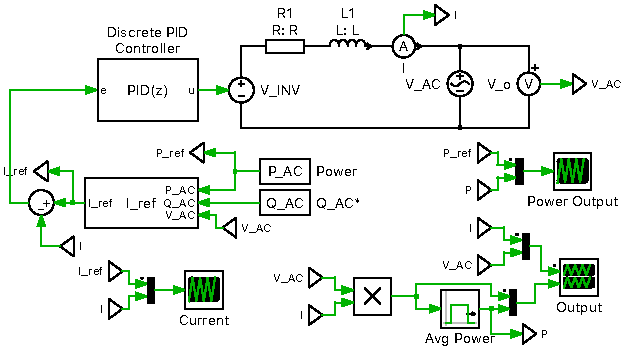
\includegraphics[width=\textwidth, height=0.4\textheight, keepaspectratio]{img/Average Time Z-C Model.pdf}
    \caption{PLECS Schematic for Average Time Discrete Controller Model}
    \label{fig:avg-time-z-c-model}
\end{figure}

\begin{figure}[ht]
    \centering{}
    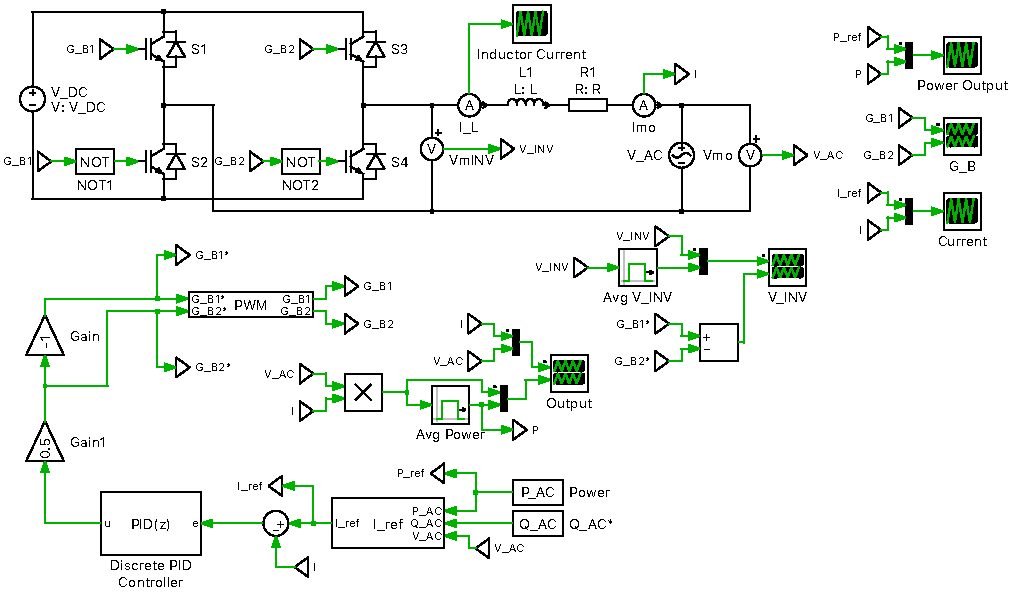
\includegraphics[width=\textwidth, height=0.4\textheight, keepaspectratio]{img/Switching Z-C Model.pdf}
    \caption{PLECS Schematic for Switching Discrete Controller Model}
    \label{fig:switching-z-c-model}
\end{figure}

The new schematic is tested with the same test as \ref{sec:cont-cc-model}.
Figure \ref{fig:avg-time-z-c-current} shows the output and reference current at power step of 0 W, $\frac{P}{2}$ W and $P$ W in average time model.
Just like the continuous controller, the output current can mostly follow the reference current.
However, at the beginning of each power transition (especially at 0 W), there is a high frequency ripple.
This is due to the sampling time of the controller not being able to respond as quickly to changes.
The negative power variants have similar patterns just with a phase shift.

\begin{figure}[ht]
    \centering{}
    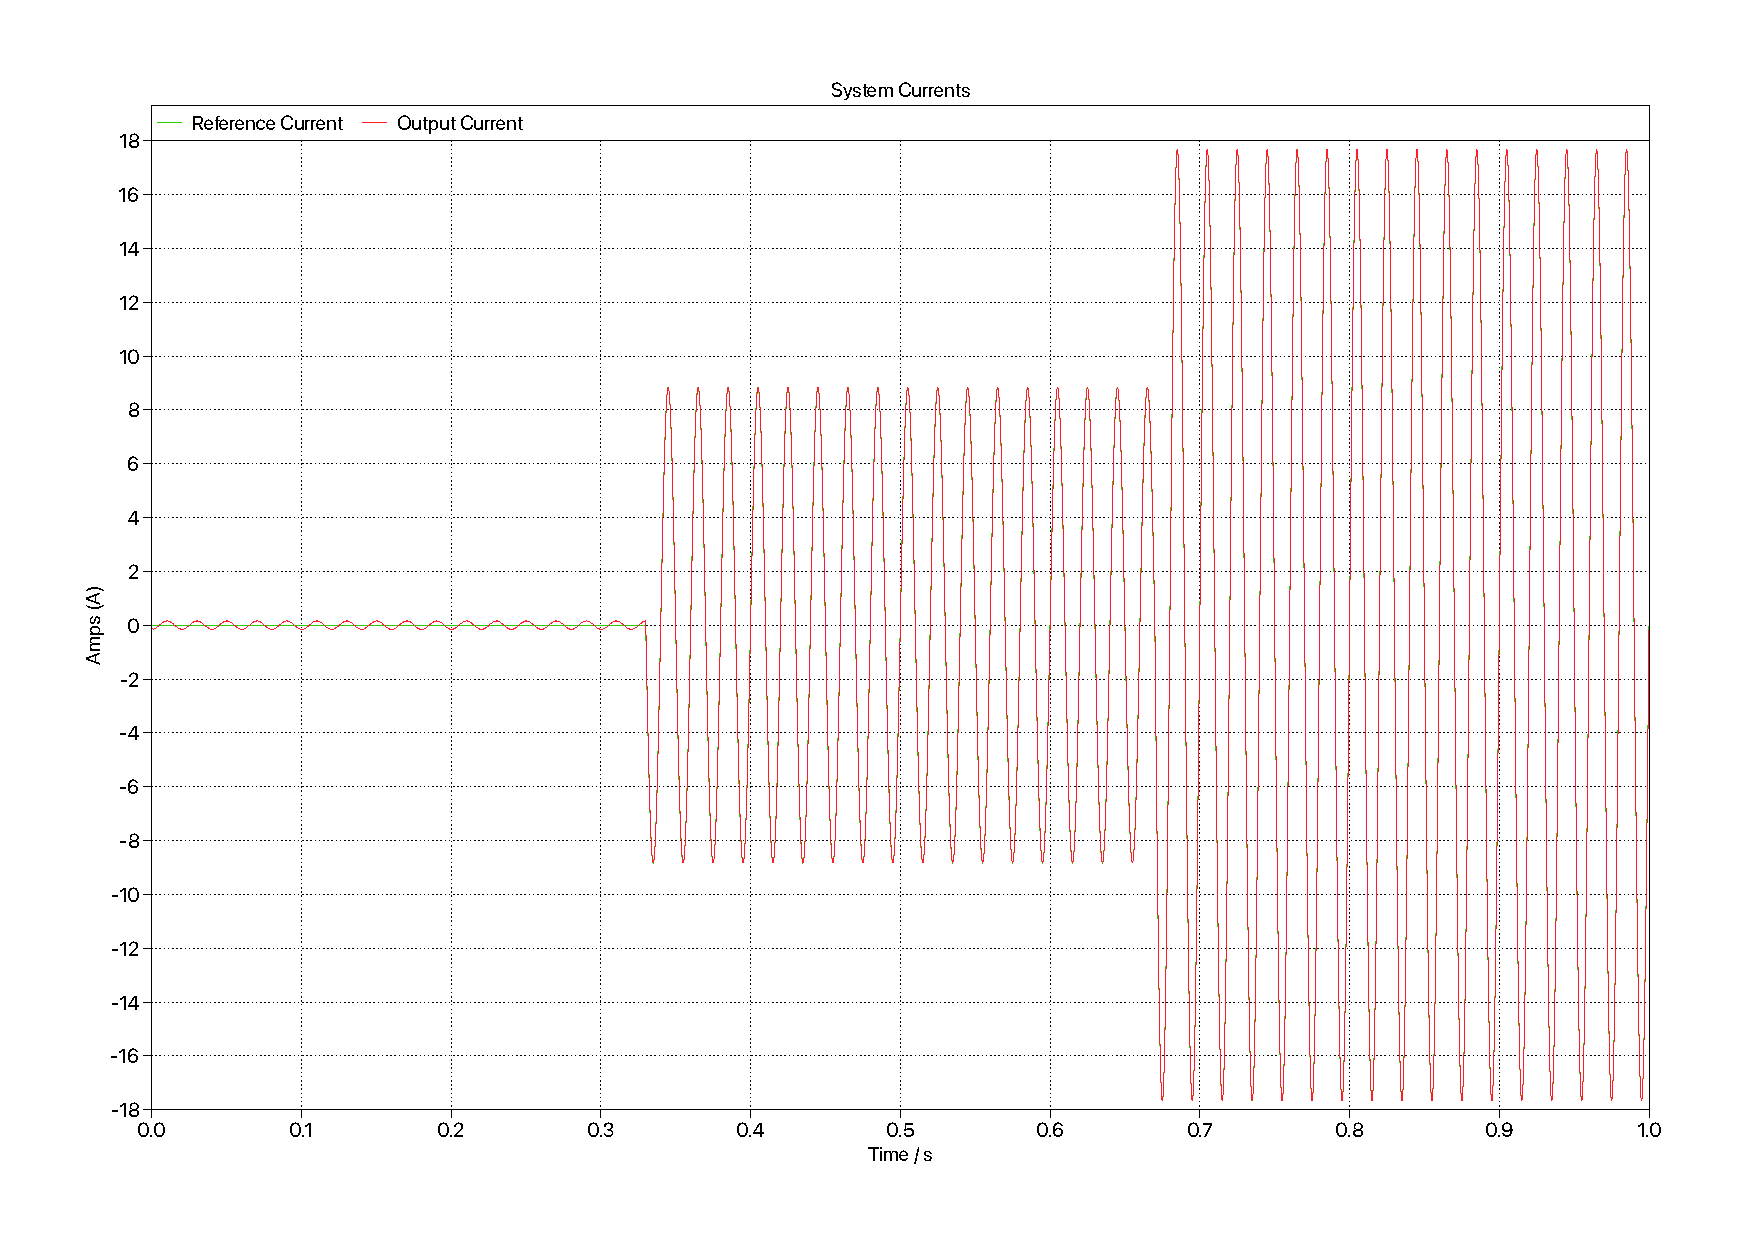
\includegraphics[width=\textwidth, height=0.4\textheight, keepaspectratio]{img/Average Time Z-C Current.pdf}
    \caption{Reference Current vs Output Current Average Time Discrete Controller Model}
    \label{fig:avg-time-z-c-current}
\end{figure}

\begin{figure}[ht]
    \centering{}
    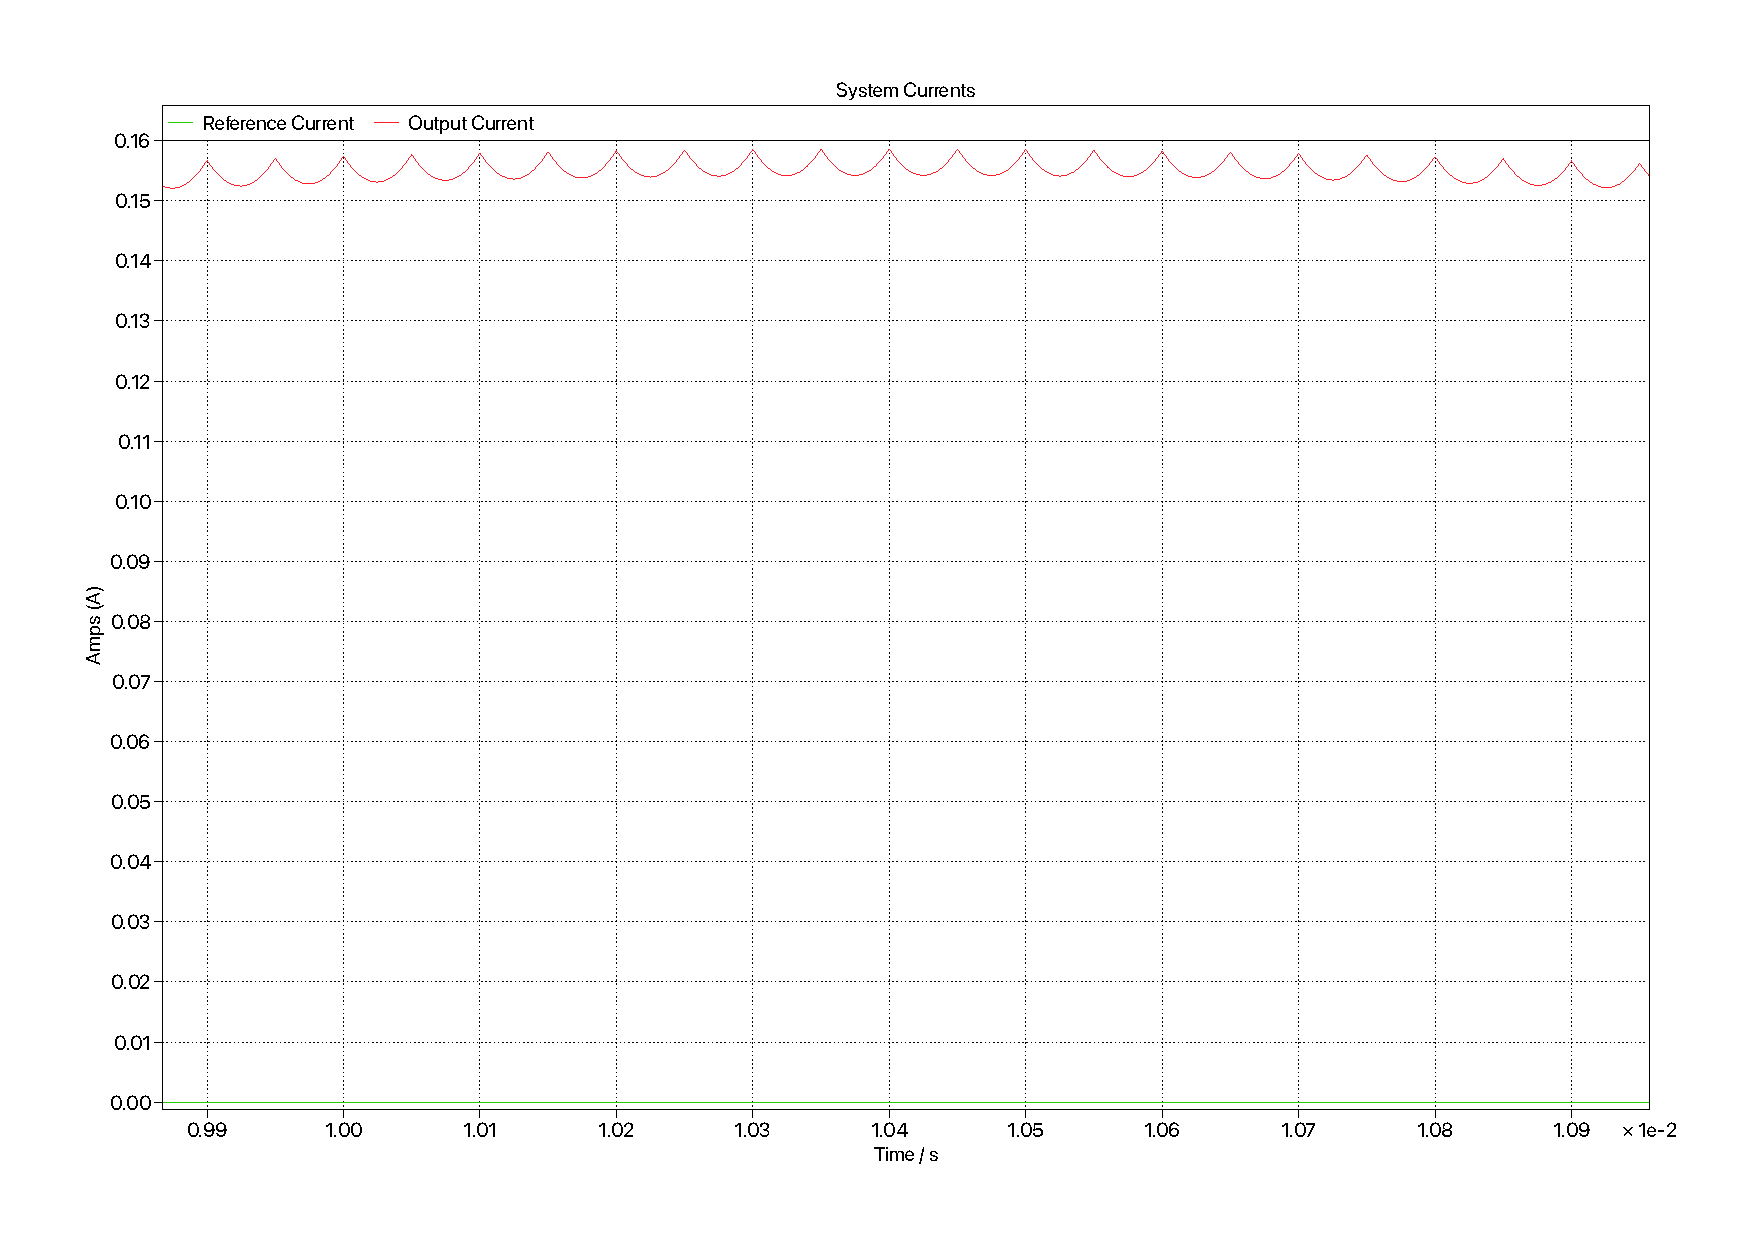
\includegraphics[width=\textwidth, height=0.4\textheight, keepaspectratio]{img/Average Time Z-C Ripple.pdf}
    \caption{Current Ripple in Output Current Average Time Discrete Controller Model}
    \label{fig:avg-time-z-c-current-ripple}
\end{figure}

The switching discrete controller model current also look similar to the continuous counterpart.
There are more current ripples compared to the continuous controller notably at 0 W.
However, this is less obvious compared to the average time model as the switching frequency is the same as the sampling frequency.
The faster reacting continuous controller is unable to follow the reference current that well as the switching frequency limiting how fast the current can change.

\begin{figure}[ht]
    \centering{}
    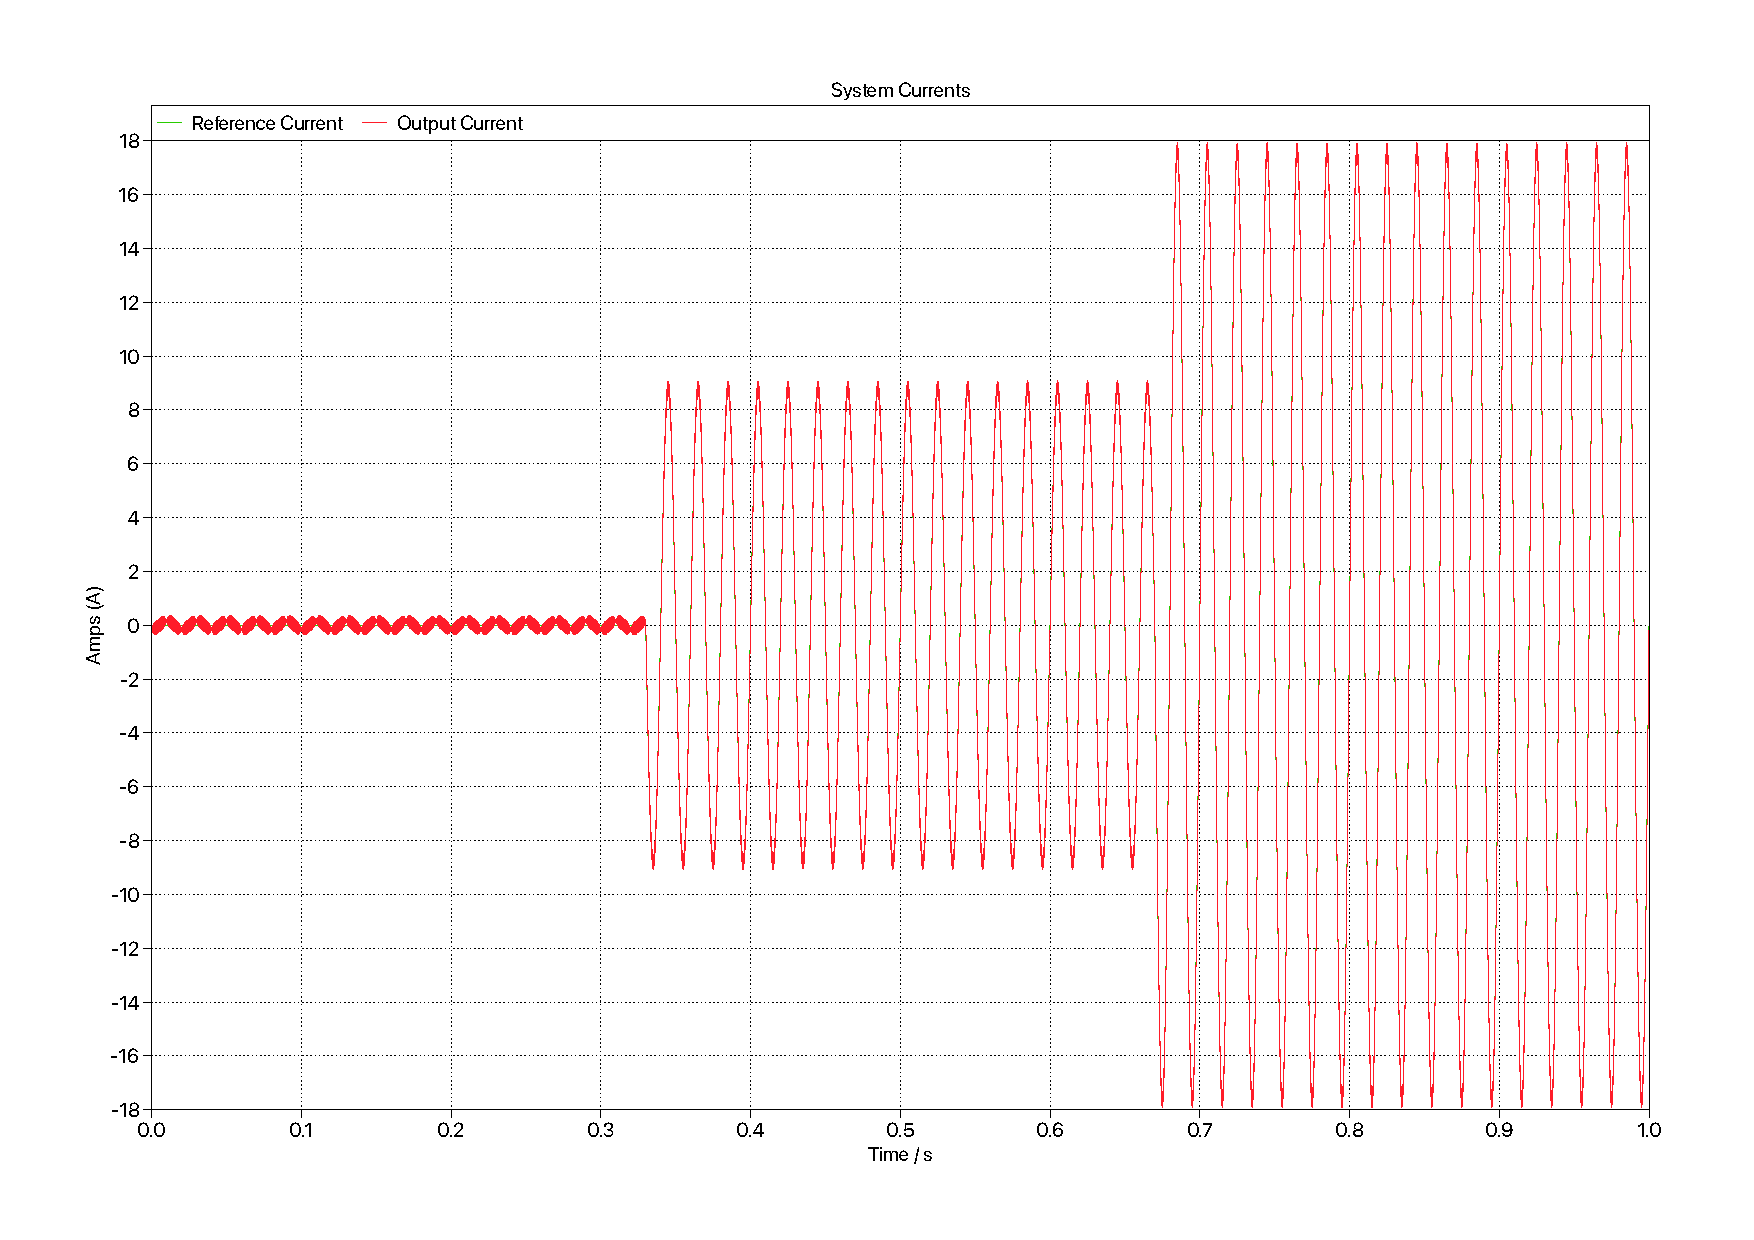
\includegraphics[width=\textwidth, height=0.4\textheight, keepaspectratio]{img/Switching Z-C Current.pdf}
    \caption{Reference Current vs Output Current Switching Discrete Controller Model}
    \label{fig:switching-z-c-current}
\end{figure}

Table \ref{tab:z-c-transient} shows the steady-state average power output compared to desired power.
The steady-state average power output is closer to the desired power than the continuous counterpart.
This is due to the sampling frequency of the discrete PID.
The continuous model has a constant over-shoot of current from the controller design.
This overshoot strays the output power away from the actual desired power, causing the performance to degrade by a little.
In the discrete model however, the controller still has an overshoot.
However, during the downtime of the controller, the current goes back down, bringing the current closer to the desired value.

\begin{table}[ht]
    \caption{Steady-State Average Power Output of Inverter}
    \label{tab:z-c-transient}
    \centering{}
    \begin{tabular}{ l l l }
        \hline
        Model        & Desired Power (W) & Output Power (W) \\
        \hline
        Average Time & $0$               & -3.333           \\
        Average Time & $1500$            & 1498.26          \\
        Average Time & $3000$            & 2999.85          \\
        \hline
        Average Time & $0$               & -3.333           \\
        Average Time & $-1500$           & -1504.92         \\
        Average Time & $-3000$           & -3006.52         \\
        \hline
        Switching    & $0$               & -3.329           \\
        Switching    & $1500$            & 1498.27          \\
        Switching    & $3000$            & 2999.86          \\
        \hline
        Switching    & $0$               & -3.329           \\
        Switching    & $-1500$           & -1504.92         \\
        Switching    & $-3000$           & -3006.52         \\
        \hline
    \end{tabular}
\end{table}

\begin{figure}[ht]
    \centering{}
    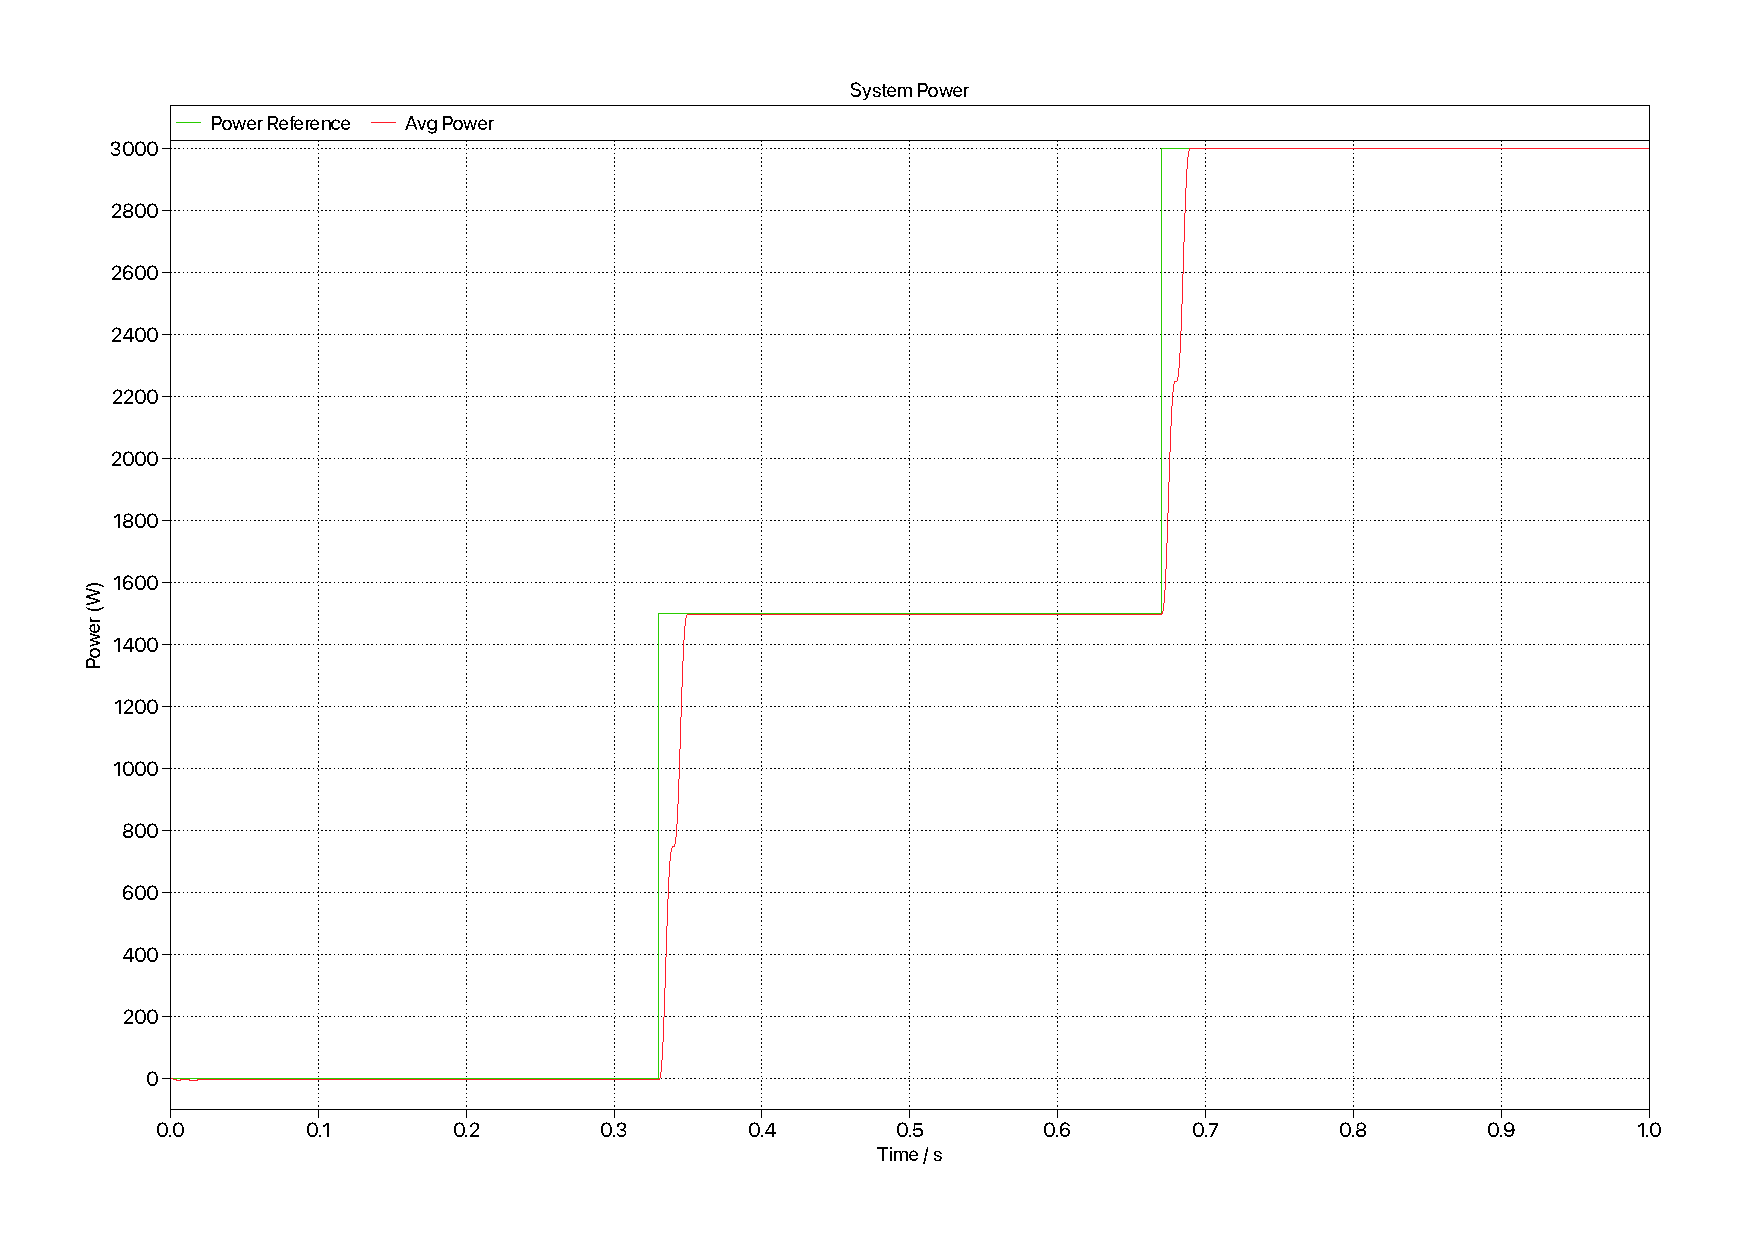
\includegraphics[width=\textwidth, height=0.4\textheight, keepaspectratio]{img/Average Time Z-C Power Positive.pdf}
    \caption{Desired Power vs Output Power Average Time Discrete Controller Positive}
    \label{fig:avg-time-z-c-power-positive}
\end{figure}

\begin{figure}[ht]
    \centering{}
    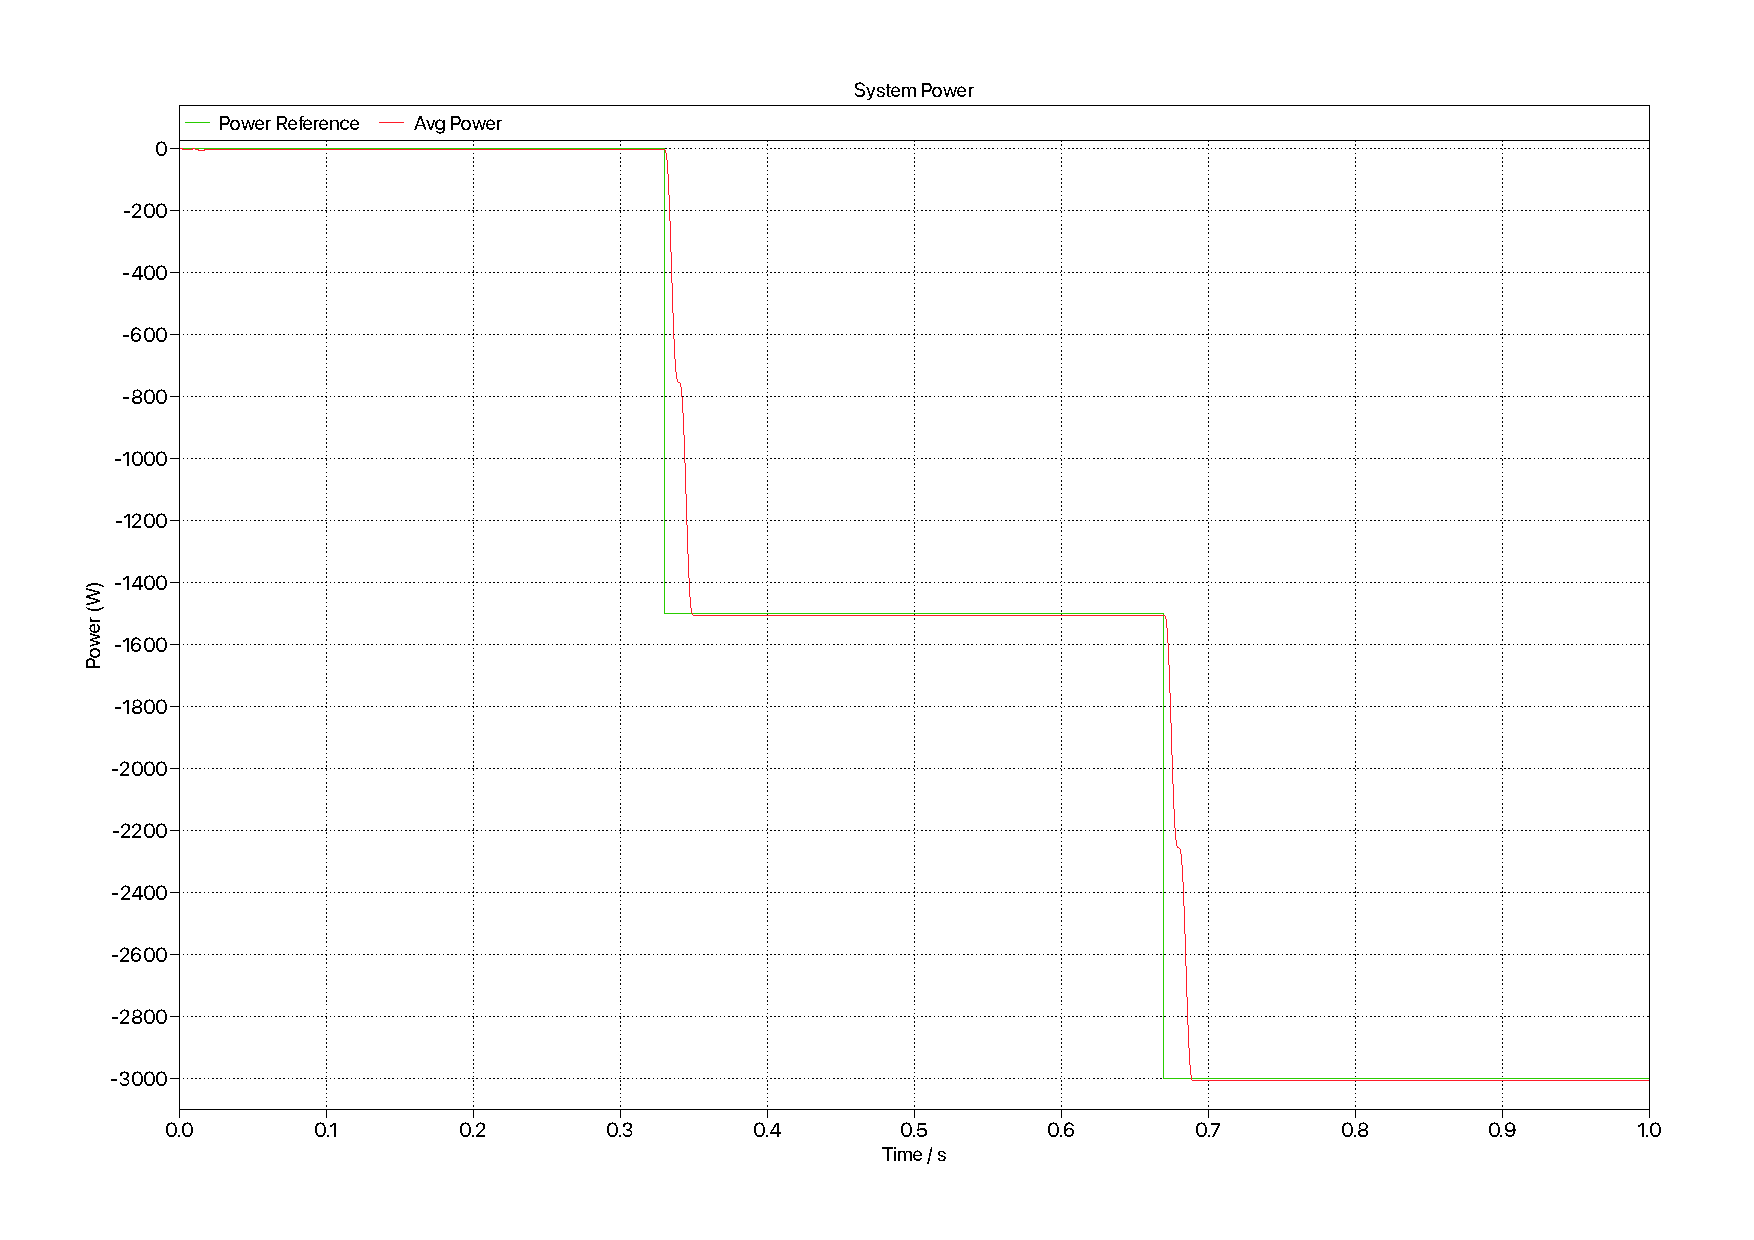
\includegraphics[width=\textwidth, height=0.4\textheight, keepaspectratio]{img/Average Time Z-C Power Negative.pdf}
    \caption{Desired Power vs Output Power Average Time Discrete Controller Negative}
    \label{fig:avg-time-z-c-power-negative}
\end{figure}

\begin{figure}[ht]
    \centering{}
    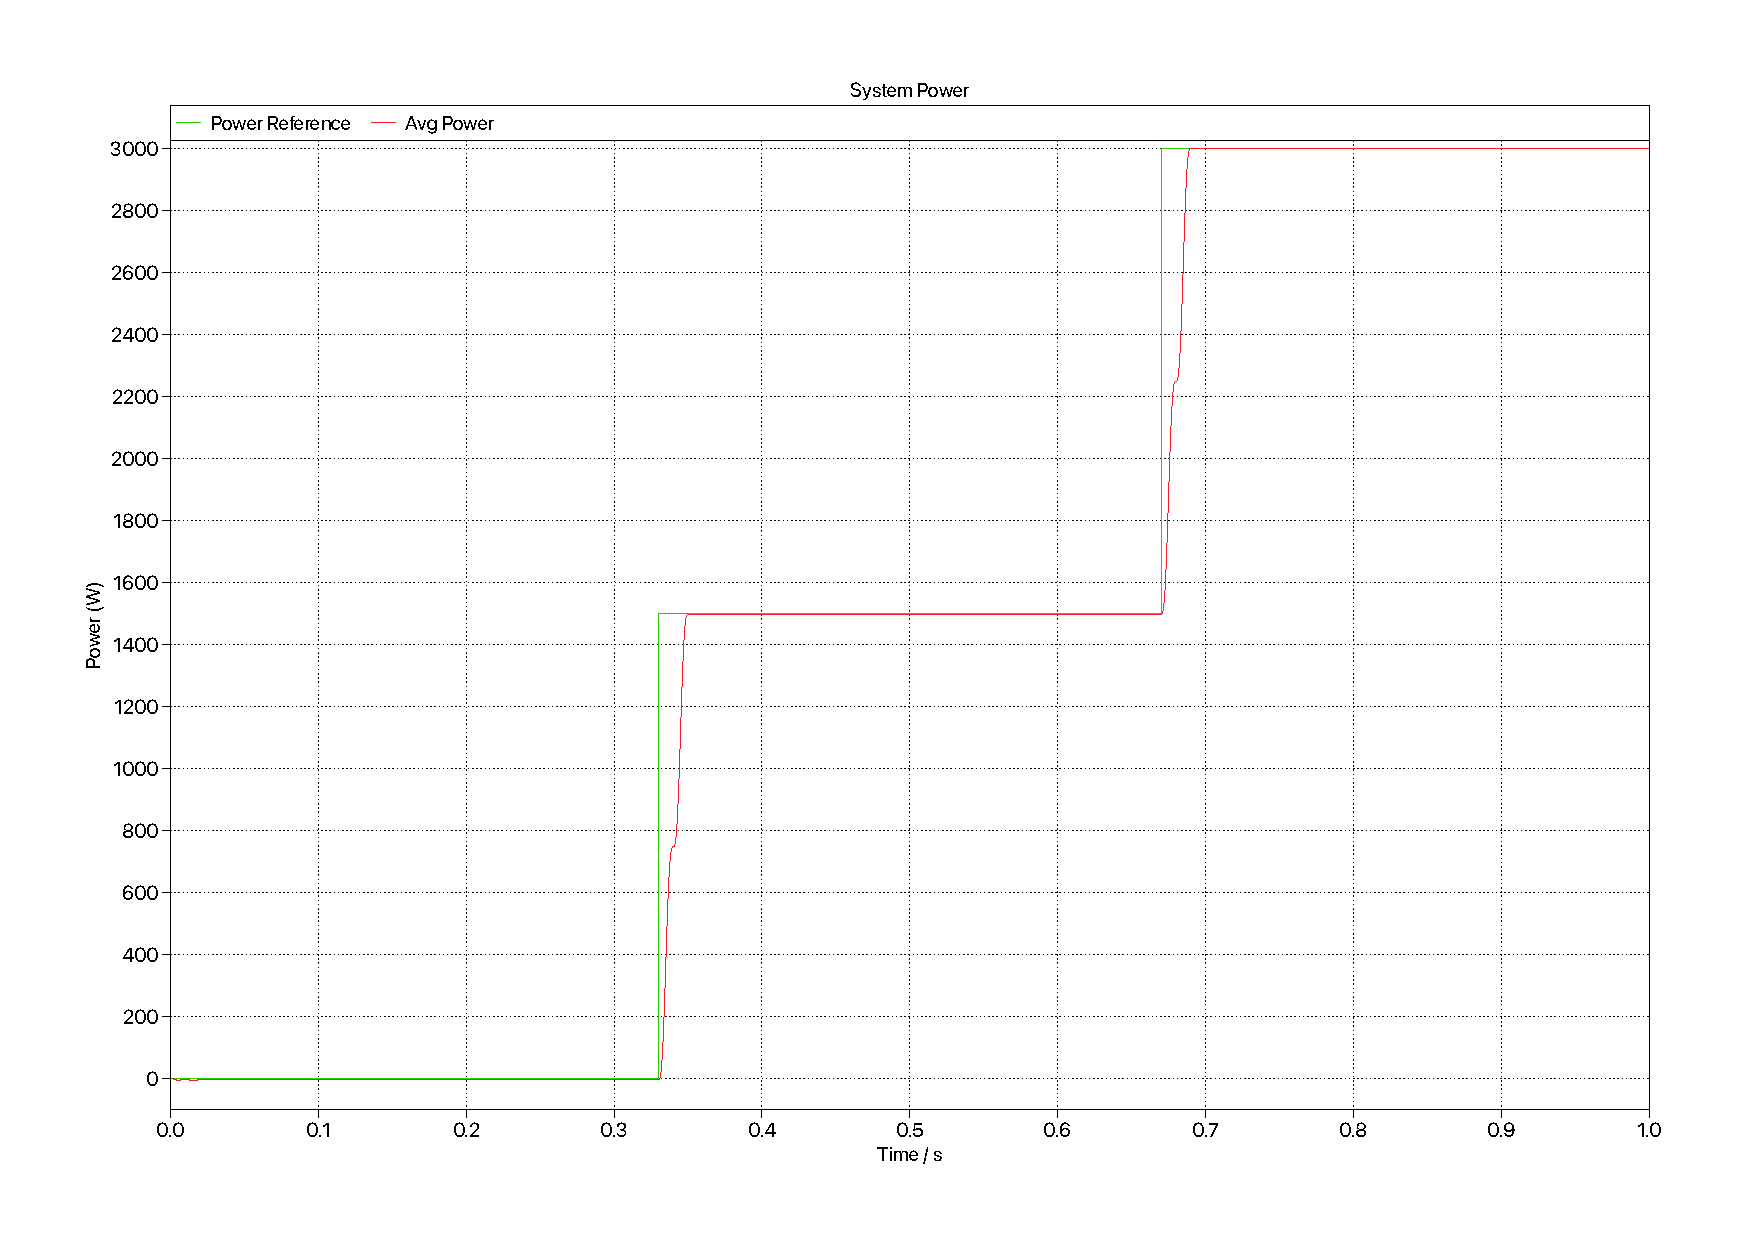
\includegraphics[width=\textwidth, height=0.4\textheight, keepaspectratio]{img/Switching Z-C Power Positive.pdf}
    \caption{Desired Power vs Output Power Switching Discrete Controller Positive}
    \label{fig:switching-z-c-power-positive}
\end{figure}

\begin{figure}[ht]
    \centering{}
    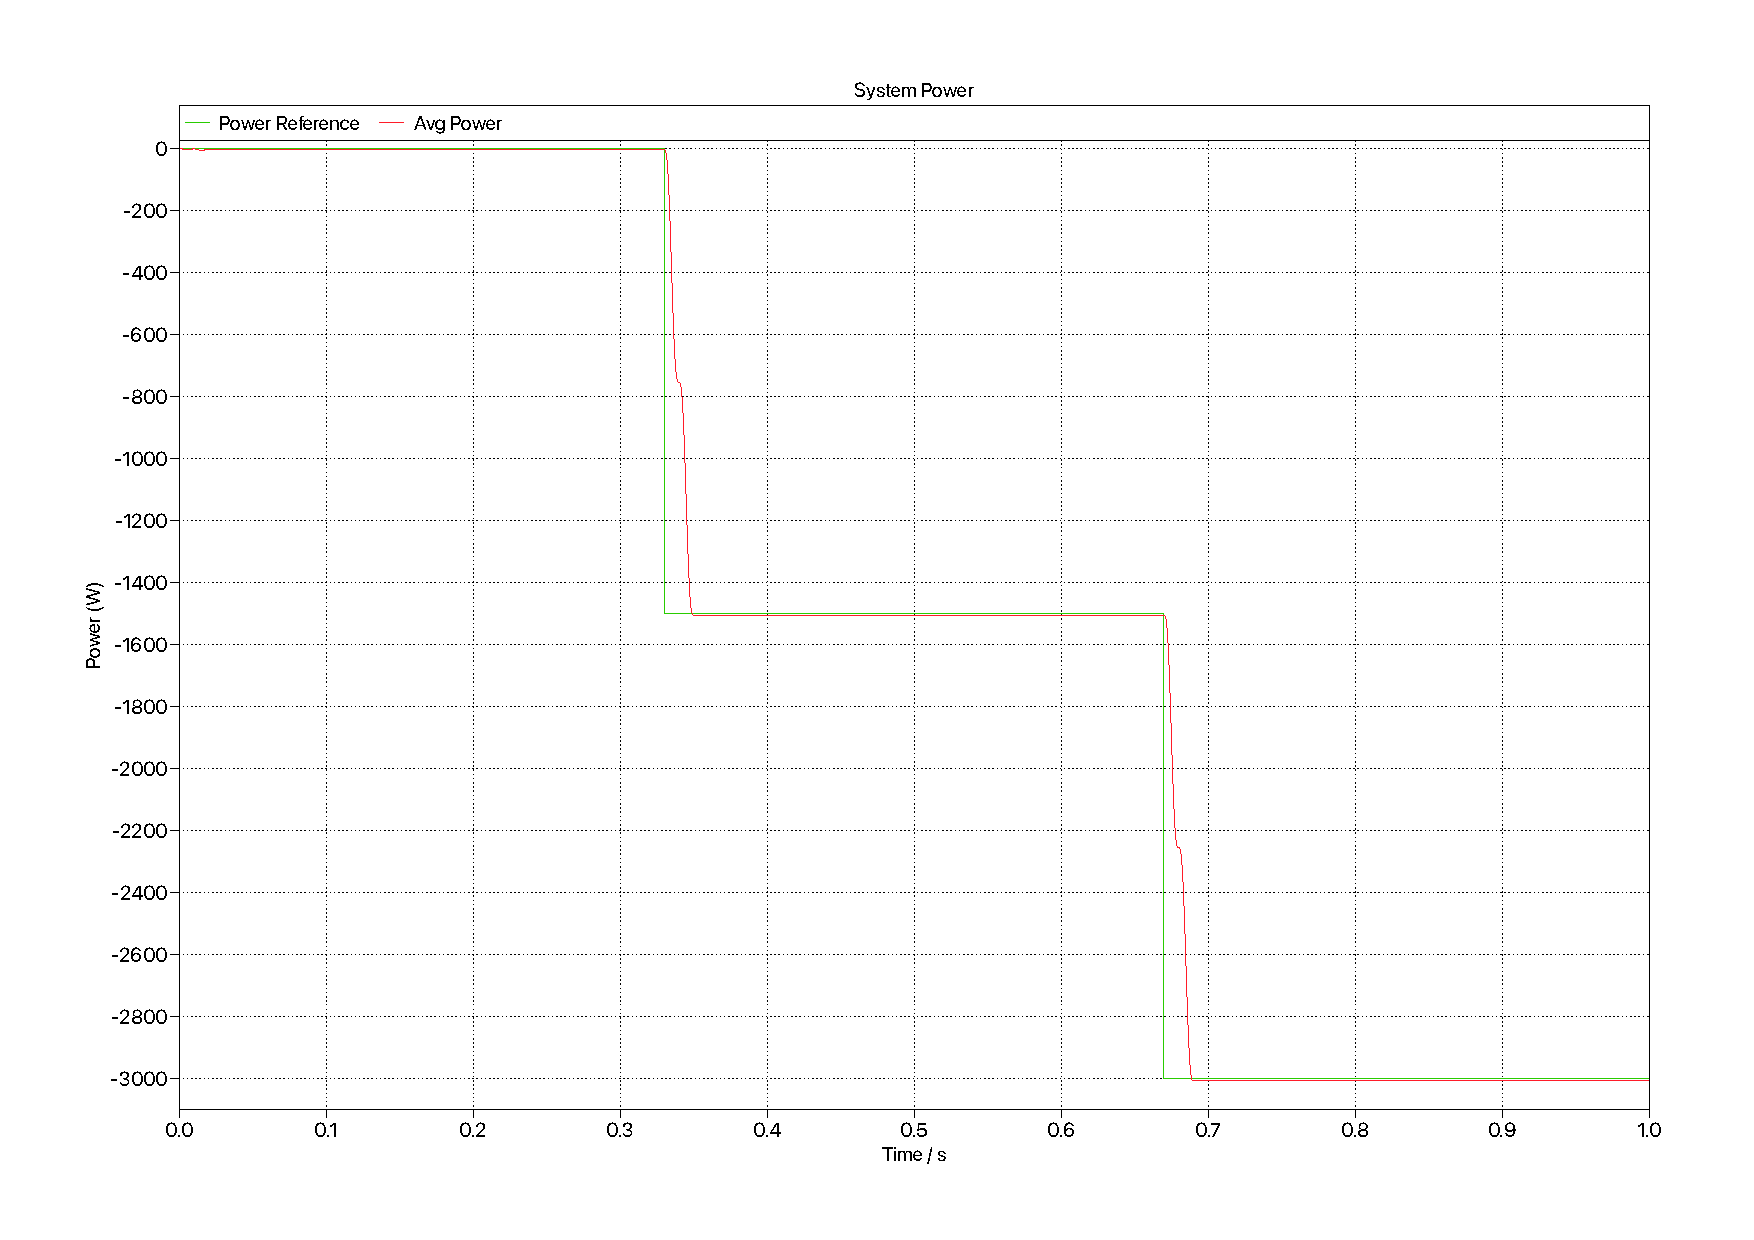
\includegraphics[width=\textwidth, height=0.4\textheight, keepaspectratio]{img/Switching Z-C Power Negative.pdf}
    \caption{Desired Power vs Output Power Switching Discrete Controller Negative}
    \label{fig:switching-z-c-power-negative}
\end{figure}

\section{Conclusion}

This coursework successfully created and simulated an inverter with good performance.
The design process starts with the design of inductor and calculation of the inverter voltage required for the power delivery.
Then, the component values calculated are simulated in 7 different models.

The first three models tests the inverter with an open loop control.
The models include the average time model without any switching, the switching model with IGBT switches and the transfer function model based on the transfer function of the inverter.
The last four are closed loop controlled inverters.
Two different types of controllers are design for these models.
The first controller is the continuous controller with transfer functions.
The second controller is the discrete controller in the z-domain.
Both of the controllers are then tested with the average time and switching models.

All the models are simulated using PLECS and their performance are evaluated.
The models are evaluated using 2 key factors.
The first factor is the output power and the second is the output current.
The PLECS simulation showed that the inverter designed is able to provide the rated power at steady-state and current below the current ripple requirements, showing the designed inverter has good performance.

\end{document}
